\documentclass{elteikthesis}

% Overleaf: keep this file named main.tex and select pdfLaTeX.
% Local build: make  (or: latexmk -pdf main.tex)
% Student metadata
\title{Migrating Spring Boot MVC Systems to Java 21 Virtual Threads: Architecture, Risks, and Engineering Guidelines}
\author{Hamed Mohamed}
\neptun{DG1EWF}
\degree{Computer Science MSc --- Software Architecture Specialisation}
\date{2026}

% Copy supervisor and programme metadata exactly from the approved topic form.
\supervisor{Dr. habil. Tamás Kozsik}
\affiliation{Associate Professor, Head of Department}

\extsupervisor{Gregory Reynolds Morse}
\extaffiliation{Lecturer and MSc in Computer Science}

\university{Eötvös Loránd University}
\faculty{Faculty of Informatics}
\department{Department of Programming Languages and Compilers}
\city{Budapest}
\logo{elte_cimer_szines}

% Draft mode displays authoring advice and policy-source examples.
% Set false before submission, then remove all remaining placeholders.
\newif\ifshowtemplateguidance
\showtemplateguidancefalse

% Guidance helpers. The retained elteikthesis class already loads xcolor,
% float, booktabs, tabularx, longtable, graphicx, pdfpages, and hyperref.
\newcommand{\TemplateGuidance}[1]{%
  \ifshowtemplateguidance
    \begin{quote}\small\color{gray!80!black}
      \textbf{Template guidance --- delete before submission.} #1
    \end{quote}
  \fi
}

\newcommand{\TemplatePrompt}[1]{%
  \ifshowtemplateguidance
    \par\noindent\textcolor{gray!80!black}{\textit{<#1>}}\par
  \fi
}

\newcommand{\MissingArtifactPage}[2]{%
  \clearpage
  \thispagestyle{empty}
  \begin{center}
    \vspace*{35mm}
    {\Huge\bfseries\textcolor{red!70!black}{MISSING REQUIRED ARTIFACT}}\\[12mm]
    {\Large\bfseries #1}\\[12mm]
    \begin{minipage}{0.75\textwidth}\centering #2\end{minipage}
  \end{center}
  \clearpage
}

\newcommand{\ResearchChain}{%
  \begin{center}
    \fbox{\parbox{0.92\textwidth}{\centering
    problem and gap $\rightarrow$ question $\rightarrow$ method
    $\rightarrow$ evidence $\rightarrow$ analysis or proof
    $\rightarrow$ result $\rightarrow$ answer $\rightarrow$ contribution}}
  \end{center}
}

\newcommand{\ContributionLedger}{%
  \begin{table}[H]
    \centering
    \caption{Contribution and responsibility boundary ledger.}
    \label{tab:contribution-ledger}
    \begin{tabularx}{\textwidth}{@{}p{0.06\textwidth}p{0.30\textwidth}p{0.28\textwidth}X@{}}
      \toprule
      \textbf{ID} & \textbf{Original substance} & \textbf{Evidence later in thesis} & \textbf{Responsibility boundary} \\
      \midrule
      C1 & Decoupling carrier unpinning from domain serialization & Chapter~\ref{ch:results} (§\ref{sec:results-rq1}, Stratum~1: 12 trials, $\Delta\text{TP} < 0.6\%$) & Student independent empirical discovery, measurement, and theoretical derivation. \\
      \addlinespace
      C2 & Silent carrier starvation via native JNI POSIX downcalls & Chapter~\ref{ch:results} (§\ref{sec:results-rq2}, Stratum~3: 27 trials, 0 JFR pinning events) & Student independent native C library implementation, telemetry design, and verification. \\
      \addlinespace
      C3 & Dual-window reporting standard and 125-run corpus audit & Chapters~\ref{ch:methodology} and~\ref{ch:results} (543 artifacts, SHA-256 verifications) & Student independent execution, open-science freeze curation, and Python validation scripts. \\
      \addlinespace
      C4 & Engineering migration framework & Chapter~\ref{ch:discussion} (§\ref{sec:migration-framework}: 5 rules, 4 refactorings, decision matrix) & Student independent synthesis based directly on empirical testbed findings. \\
      \bottomrule
    \end{tabularx}
  \end{table}
}


\begin{document}
\documentlang{english}

\hypersetup{pageanchor=false}
\maketitle
\pagenumbering{gobble}

% Export the approved MSc topic-registration form to this exact filename.
\IfFileExists{approved-topic-registration.pdf}{%
  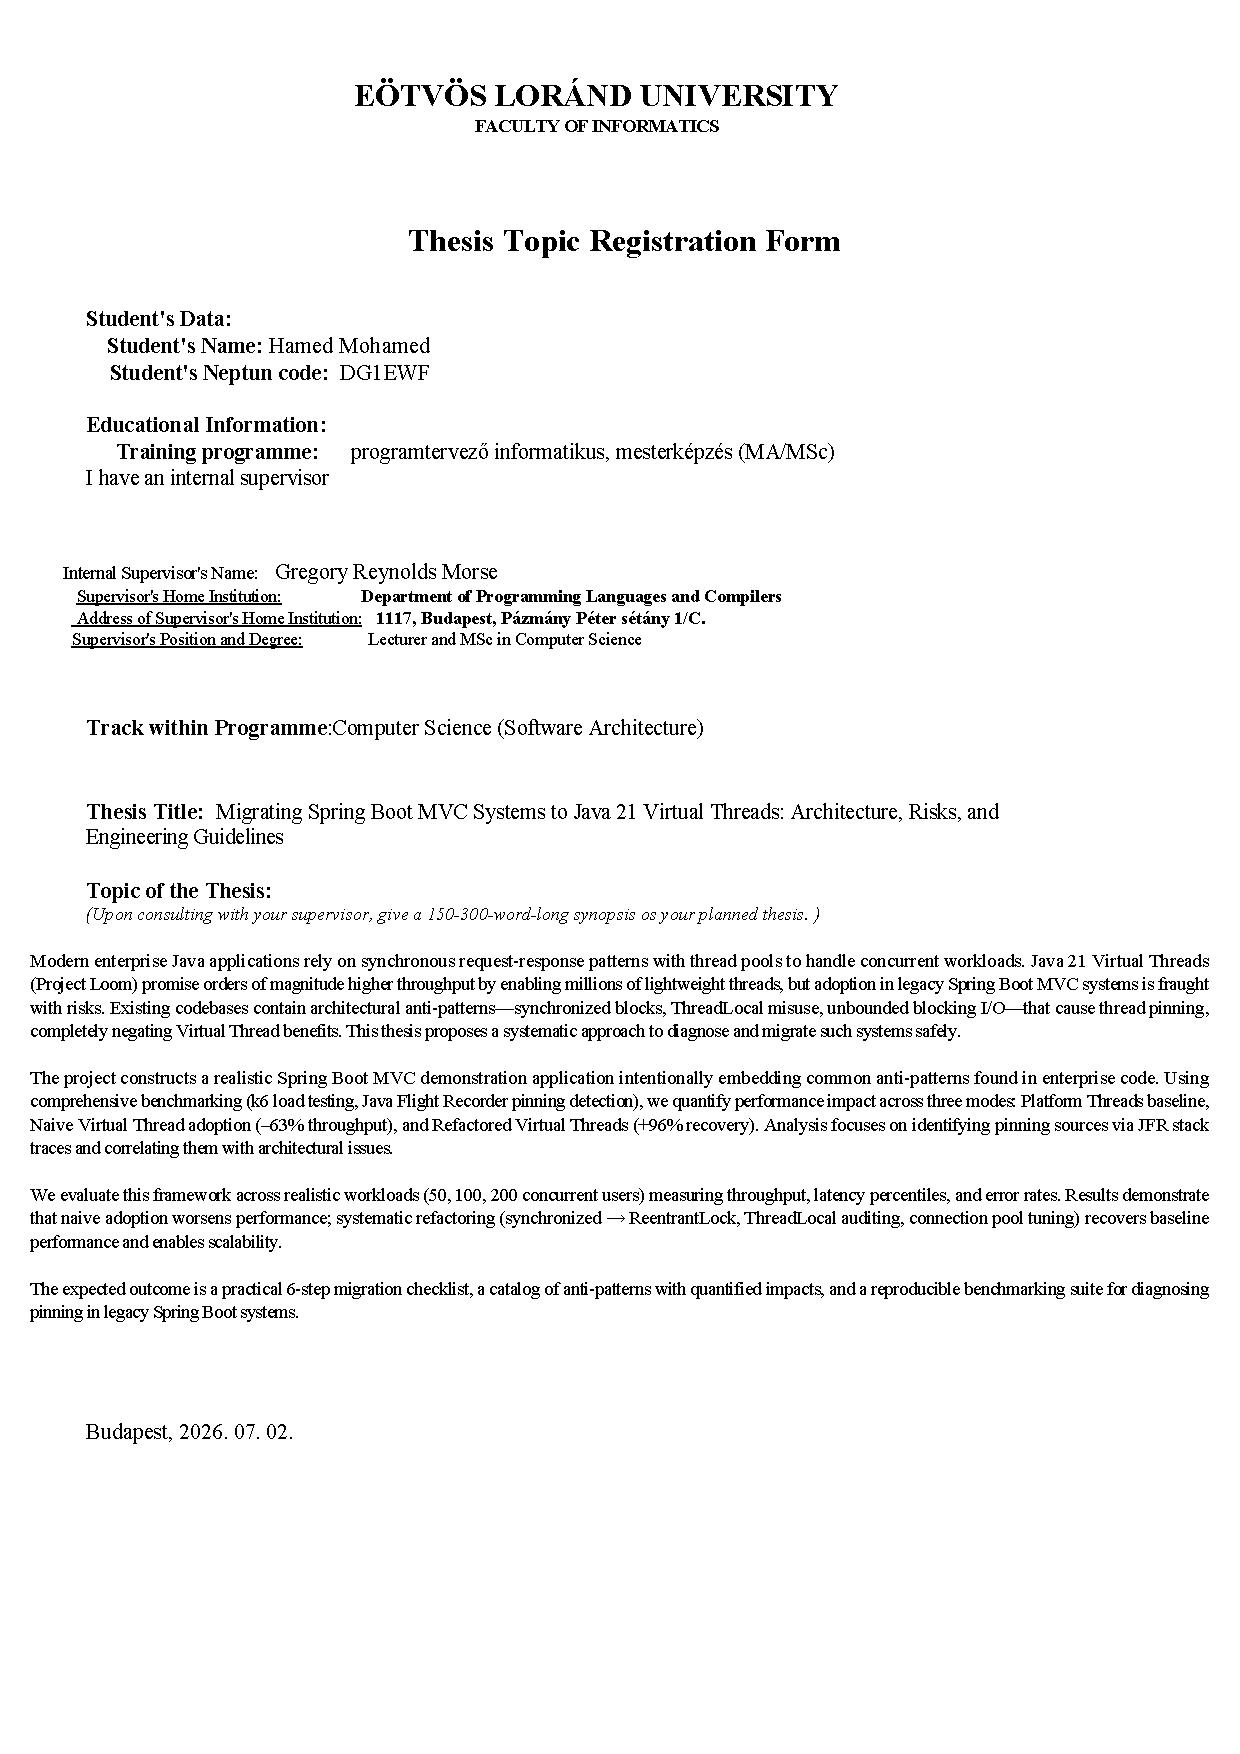
\includepdf[pages=-,pagecommand={\thispagestyle{empty}}]{approved-topic-registration.pdf}
}{%
  \MissingArtifactPage{Approved MSc Thesis Topic Registration Form}{%
    Export the approved form as \texttt{approved-topic-registration.pdf} and upload it
    beside \texttt{main.tex}. Verify programme, specialisation, title, supervisor,
    contribution, and dates against the final thesis.}
}

\ifshowtemplateguidance
  \chapter*{Authoring Control --- Delete Before Submission}

\TemplateGuidance{This page is a planning aid. Current ELTE IK rules override it.
The six review areas are holistic; the 30-point weights below come from the
supplied point-by-point review form and do not create an automatic score-to-grade
conversion.}

\ResearchChain

\begin{table}[H]
  \centering
  \caption*{Official review areas and point-by-point planning weights}
  \begin{tabularx}{\textwidth}{@{}p{0.08\textwidth}X p{0.15\textwidth}X@{}}
    \toprule
    \textbf{No.} & \textbf{Review area} & \textbf{Weight} & \textbf{Primary locations} \\
    \midrule
    I & Research scope and goals & 4 / 30 & Introduction; topic traceability \\
    II & Development of the topic & 5 / 30 & Related Work; Background; decision narrative \\
    III & Methods & 9 / 30 & Methodology; procedure or artifact; validity and reproducibility \\
    IV & Results and contribution & 9 / 30 & Results; Discussion; Conclusion \\
    V & Presentation, language and structure & 2 / 30 & Whole thesis; figures; references; boundaries \\
    VI & Preparation process & 1 / 30 & Supervision and milestone evidence, including records outside the thesis \\
    \bottomrule
  \end{tabularx}
\end{table}

\begin{table}[H]
  \centering
  \caption*{Research-mode routing}
  \begin{tabularx}{\textwidth}{@{}p{0.23\textwidth}X X@{}}
    \toprule
    \textbf{Mode} & \textbf{Primary evidence} & \textbf{Critical validity checks} \\
    \midrule
    Theoretical/formal & Definitions, models, lemmas, proofs, counterexamples, certificates & Assumptions, quantifiers, completeness, edge cases, independent proof checking \\
    Empirical ML/data & Licensed data, splits, code, models, configurations, predictions, measurements & Provenance, leakage, fair tuning, baselines, seeds, uncertainty, robustness, ablations \\
    Engineering/system & Source, builds, tests, workloads, traces, measurements & Correctness, rationale, workload realism, fair comparison, security, usability \\
    Human-subject/user study & Protocol, instruments, approvals, anonymised data, coding and analysis & Consent, privacy, sampling, construct validity, bias, missing data, limits \\
    Simulation / numerical & Model, solver, parameters, initial conditions, logs, convergence evidence & Model validity, numerical stability, tolerance, convergence, calibration, sensitivity \\
    Qualitative/design & Cases, artefacts, protocol, coding records, reflexive documentation & Selection, triangulation, coding reliability, researcher influence, coverage, transfer limits \\
    \bottomrule
  \end{tabularx}
\end{table}

\TemplateGuidance{Choose three final-examination subjects related to the thesis and
master their concepts. Integrate relevant ideas naturally; do not create artificial
``Exam Topic 1/2/3'' headings. Keep the editable source, PDF, artifacts, data or
proofs, logs, and process records on the same final revision.}

\fi

\cleardoublepage
\chapter*{Abstract}
This dissertation examines the architectural, performance, and operational implications of migrating Spring Boot MVC systems to Java~21 Virtual Threads (Project Loom, JEP~444). Although virtual threads decouple Java threads from OS kernel threads to prevent web-tier pool exhaustion, migration remains bounded by the \emph{Schedulability Fallacy}: user-mode multiplexing does not remove application serialization, downstream resource caps, or native carrier captivity.

A Spring Boot 3.5.12 MVC testbed was evaluated across 125 physical runs in eight strata, with k6 streams, Java Flight Recorder (JFR) traces, and OS telemetry SHA-256 verified and analyzed under a dual-window steady-state standard. In the tested Java~21 condition, blocking inside \texttt{synchronized} generated 108 qualifying \texttt{jdk.VirtualThreadPinned} events ($\ge 20\text{ ms}$); refactoring to \texttt{ReentrantLock} produced zero qualifying events with similar throughput ($1.956$ vs.\ $1.967\text{ req/s}$, $0.56\%$ delta; $\mu \approx 2.0\text{ req/s}$) and a 20-fold larger between-trial dispersion ($\sigma = 16.34$ vs.\ $0.82\text{ ms}$). Direct JNI POSIX \texttt{nanosleep()} occupied carriers with $\approx 1\%$ process CPU and zero JFR pinning events. Holding JDBC connections across blocking operations empirically validated the Downstream Bottleneck Shift Law ($X_{\text{max}} = K/T_{\text{hold}}$) with zero qualifying pins.

Synthesizing these findings yields the \emph{Three-Tier Concurrency Taxonomy}, five architectural rules, four refactoring patterns, and a migration decision matrix.\footnote{Codex (GPT-6.2 Sol) assisted with aligning the name of the migration decision matrix; Google Gemini assisted with editorial condensation and English--Hungarian parity calibration.}

\bigskip
\noindent\textbf{Keywords:} Project Loom, Thread Pinning, Carrier Starvation, Java Flight Recorder, Connection Pooling.

\cleardoublepage
\chapter*{Kivonat}
Jelen diplomamunka a Java~21 virtuális szálak (Project Loom, JEP~444) Spring Boot MVC rendszerekben történő bevezetésének architekturális, teljesítménybeli és üzemeltetési hatásait vizsgálja. Bár a virtuális szálak szétválasztják a Java szálakat az OS platformszálaitól -- megelőzve a webes szálkészlet-kimerülést --, a migrációt továbbra is korlátozza az \emph{Ütemezhetőségi Tévedés}: a felhasználói szintű multiplexelés nem szünteti meg az alkalmazásszintű sorosítást, a háttérerőforrások korlátait vagy a natív hordozófoglalást.

Egy Spring Boot 3.5.12 MVC tesztrendszeren 125 fizikai mérést hajtottunk végre nyolc rétegben; a k6 naplókat, a Java Flight Recorder (JFR) nyomkövetéseket és az OS telemetriát SHA-256 ellenőrzéssel és kétablakos egyensúlyi kiértékeléssel vizsgáltuk. A vizsgált Java~21 feltételek között a \texttt{synchronized} blokkolás 108 küszöbérték feletti ($\ge 20\text{ ms}$) \texttt{jdk.VirtualThreadPinned} eseményt okozott; a \texttt{ReentrantLock} nulla küszöbérték feletti esemény mellett hasonló átviteli sebességet ($1.956$ vs.\ $1.967\text{ req/s}$, $0.56\%$-os eltérés; $\mu \approx 2.0\text{ req/s}$) és közel 20-szor nagyobb futások közötti szórást ($\sigma = 16.34$ vs.\ $0.82\text{ ms}$) adott. A közvetlen JNI POSIX \texttt{nanosleep()} $\approx 1\%$-os folyamat-CPU mellett nulla JFR rögzítési eseménnyel foglalta le a hordozószálat. A blokkolás alatti JDBC-kapcsolat-tartás nulla rögzítési esemény mellett igazolta a Lefelé Tolódó Szűk Keresztmetszet Törvényét ($X_{\text{max}} = K/T_{\text{hold}}$).

Az eredményekre épül a \emph{Háromszintű Párhuzamossági Taxonómia}, öt architekturális szabály, négy refaktorálási minta és egy migrációs döntési mátrix.\footnote{A migrációs döntési mátrix megnevezésének egységesítésében a Codex (GPT-6.2 Sol), a tömörítésben és a magyar--angol egyezőség ellenőrzésében a Google Gemini segített.}

\bigskip
\noindent\textbf{Kulcsszavak:} Project Loom, Szálrögzítés, Hordozó-kiéheztetés, Java Flight Recorder, Kapcsolatkészlet-méretezés.

\cleardoublepage
\hypersetup{pageanchor=true}
\pagenumbering{arabic}
\setcounter{page}{1}
\tableofcontents

\chapter{Introduction}
\label{ch:introduction}

\section{Programme and Specialisation Fit}
\label{sec:programme-fit}

This master's dissertation is submitted in partial fulfillment of the requirements for the degree of \emph{Master of Science in Computer Science} within the \emph{Software Architecture Specialisation} at the Faculty of Informatics, Eötvös Loránd University (ELTE), Budapest~\cite{elteikMscRules}. The research was conducted under the institutional auspices of the Department of Programming Languages and Compilers, under the joint supervision of Associate Professor Dr.~habil.\ Tamás Kozsik (Head of Department) and external thesis advisor Gregory Reynolds Morse (Lecturer and MSc in Computer Science)~\cite{morseMscGuidance}, pursuant to approved MSc thesis topic registration \texttt{IK-ZVMSC\_EN2\_155}.

The dissertation directly addresses three core subject areas of the MSc curriculum and final examination syllabus:
\begin{enumerate}
  \item \textbf{Software Architecture and Scalable Enterprise Systems:} Evaluating request-dispatching topologies, concurrency bounding, connection-pool queueing dynamics, and architectural boundary preservation when migrating synchronous enterprise web services from OS-managed thread pools to lightweight user-space threads.
  \item \textbf{Advanced Java Programming and Runtime Internals:} Deconstructing Java Virtual Machine (JVM) execution mechanics, continuation capture, intrinsic monitor synchronization (\texttt{synchronized}), explicit lock synchronization (\texttt{java.\allowbreak util.\allowbreak concurrent.\allowbreak locks.\allowbreak ReentrantLock}), the AbstractQueuedSynchronizer (AQS) framework, and the OpenJDK HotSpot runtime transition from Java~21 LTS (JEP~444~\cite{JEP444}) to Java~24 (JEP~491~\cite{JEP491}).
  \item \textbf{Systems Engineering, Project Management, and Empirical Rigour:} Designing reproducible benchmark suites, managing experimental artifacts, instituting open-science data freezes with cryptographic integrity, and establishing compliance with academic governance standards, including ELTE Dean's Directive~1/2026~\cite{elteikAiPolicy}.
\end{enumerate}

\section{Motivation and Research Problem}
\label{sec:motivation-problem}

For more than two decades, enterprise Java backend architectures have overwhelmingly relied upon the synchronous, \emph{thread-per-request} paradigm. Standardized by the Java Servlet API and realized in production web servers such as Apache Tomcat~\cite{TomcatReference} and Spring Framework Model-View-Controller (MVC) containers~\cite{SpringReference}, this architecture assigns each incoming HTTP connection to a dedicated worker thread. This paradigm provides immense developer ergonomics: sequential imperative code execution, natural diagnostic stack traces, implicit request-scoped context propagation via \texttt{ThreadLocal}, and seamless integration with synchronous blocking persistence APIs such as JDBC and HikariCP~\cite{HikariCPReference}.

However, this architecture historically rested upon an inflexible foundation: a strict $1:1$ mapping between Java threads (\texttt{java.lang.Thread}) and operating system (OS) kernel platform threads (such as POSIX \texttt{pthread}s). Because platform threads allocate heavyweight virtual memory stacks (defaulting to $1\,024\text{ KB}$ per thread in HotSpot via \texttt{-Xss1m}) and incur preemptive kernel context-switching latency, enterprise containers strictly bound concurrency using fixed thread pools (e.g., Tomcat's default \texttt{maxThreads = 200}). Under high concurrency or during downstream I/O latency spikes, worker thread pools exhaust rapidly, inducing connection backlog queueing, exponential latency escalation, and catastrophic server timeouts.

To circumvent platform thread exhaustion, reactive, event-driven architectures (such as Spring WebFlux, Project Reactor, and Netty) emerged during the 2010s. By multiplexing concurrent connections across a tiny pool of non-blocking event-loop threads matching CPU core counts, reactive systems eliminated thread pool exhaustion. Yet this efficiency imposed severe cognitive and operational costs: the abandonment of imperative control flow in favor of monadic functional pipelines (\texttt{Mono}, \texttt{Flux}), fragmented stack traces that obscure production debugging, and fundamental architectural friction when interfacing with blocking relational database drivers (JDBC).

The delivery of \textbf{Project Loom} in \textbf{Java 21 LTS} via \textbf{JEP 444}~\cite{JEP444} was engineered to eliminate this trade-off. Virtual Threads introduce lightweight, user-mode threads managed directly by the JVM runtime under an $M:N$ scheduling architecture:
\begin{itemize}
  \item Millions of ephemeral virtual threads ($M$) can be instantiated with minimal initial memory footprints ($\approx 1\text{ KB}$), storing their call frames as \texttt{Continuation} objects directly on the garbage-collected Java heap.
  \item A small pool of OS platform threads ($N$), managed by a work-stealing HotSpot \texttt{ForkJoinPool} (\texttt{DEFAULT\_SCHEDULER}), acts as \emph{carrier threads} that physically execute instructions on CPU cores.
  \item When a virtual thread executes a blocking operation within standard Java libraries (such as socket I/O, \texttt{Thread.sleep()}, or \texttt{ReentrantLock.lock()}), the runtime captures its continuation frames to the heap and \emph{unmounts} the virtual thread from its carrier, freeing the underlying OS thread to execute other ready virtual threads.
\end{itemize}

In Spring Boot 3.2.0 and later (evaluated in this dissertation on Spring Boot 3.5.12), enabling virtual threads requires only a single configuration property:
\begin{verbatim}
spring.threads.virtual.enabled: true
\end{verbatim}
Setting this property configures Tomcat to dispatch incoming HTTP requests to an ephemeral virtual thread created by \texttt{Executors.\allowbreak newVirtualThread\allowbreak PerTaskExecutor()}.

\subsection{The Virtual Thread Bottleneck Fallacy}
The effortless activation of virtual threads catalyzed a widespread industry misconception that this dissertation defines as \textbf{The Virtual Thread Bottleneck Fallacy}. This fallacy presumes that the primary limiting factor in enterprise backend performance is always web-tier container thread pool concurrency, and that enabling virtual threads universally eliminates concurrency bottlenecks, drastically cuts latencies, and delivers immediate order-of-magnitude throughput gains.

In reality, removing the platform thread ceiling does not eliminate performance bottlenecks; rather, it shifts the operational pressure points deeper into the application architecture:
\begin{enumerate}
  \item \textbf{Domain Serialization Ceiling:} Enterprise workflows frequently contain shared mutable state protected by mutual exclusion (such as Java intrinsic monitors, explicit locks, or database table locks). By Amdahl's Law~\cite{Amdahl1967}, if an operation contains a serial duration $D$, the maximum system service rate is fundamentally bounded by $\mu = 1/D$, irrespective of whether requests are served by platform threads or virtual threads.
  \item \textbf{Carrier Pinning Hazards:} In Java 21, when a virtual thread blocks inside an intrinsic monitor (\texttt{synchronized} block or method), the JVM runtime cannot unmount the virtual thread from its carrier thread. This phenomenon---\emph{monitor pinning}---locks the underlying OS platform thread in place. Under concurrent load, carrier threads are rapidly exhausted, starving the entire scheduler.
  \item \textbf{Silent Native Carrier Captivity:} When a virtual thread invokes native code via the Java Native Interface (JNI), blocking POSIX system calls (e.g., \texttt{nanosleep()}) execute entirely outside HotSpot continuation management. The OS carrier thread is captured in an unmanaged wait state, starving the virtual thread pool without generating any Java Flight Recorder (JFR) pinning telemetry.
  \item \textbf{Downstream Connection Pool Exhaustion:} In relational persistence, holding a database connection across a blocking operation shifts queueing entirely to the JDBC connection pool. Even though virtual threads unmount cleanly without pinning carrier threads, total throughput is capped by pool capacity ($X_{\text{max}} = K / T_{\text{hold}}$), causing queue formation at the database pool checkout tier.
\end{enumerate}

\section{Research Goals, Questions, and Hypotheses}
\label{sec:research-questions}

To establish a rigorous, empirical systems investigation into these phenomena, this dissertation addresses two canonical Research Questions:

\bigskip

\noindent\fbox{%
\parbox{\dimexpr\textwidth-2\fboxsep-2\fboxrule\relax}{%
\textbf{Research Question 1 (RQ1):}\\
\emph{How does synchronization (specifically monitor pinning) interact with carrier-thread availability, application-level serialization, and runtime throughput in Java 21 Spring Boot MVC systems?}%
}}

\bigskip

\noindent\fbox{%
\parbox{\dimexpr\textwidth-2\fboxsep-2\fboxrule\relax}{%
\textbf{Research Question 2 (RQ2):}\\
\emph{What architectural risks---including native boundaries, connection pool management, context propagation, and observability limits---must engineering teams evaluate before enabling Virtual Threads in existing Spring Boot MVC systems?}%
}}

\bigskip

To ensure answerability and rigorous empirical evaluation, Table~\ref{tab:research-questions} operationalizes each research question into concrete treatments, hypotheses, and required evidentiary criteria.

\begin{table}[H]
  \centering
  \small
  \caption{Research questions, operational deconstruction, and intended evidence.}
  \label{tab:research-questions}
  \begin{tabularx}{\textwidth}{@{}p{0.07\textwidth}p{0.26\textwidth}p{0.26\textwidth}X@{}}
    \toprule
    \textbf{ID} & \textbf{Operational Focus} & \textbf{Treatment \& Variables} & \textbf{Intended Evidentiary Criteria} \\
    \midrule
    RQ1 & Carrier pinning vs.\ domain serialization ceiling & Factorial matrix: Tomcat platform vs.\ virtual threads; \texttt{synchronized} vs.\ \texttt{ReentrantLock} vs.\ no-lock; Java~21 LTS vs.\ Java~24 (JEP~491). & JFR \texttt{jdk.VirtualThreadPinned} events (108 to 0); steady-state throughput ($1.956$ vs.\ $1.967\text{ req/s}$); Amdahl ceiling proof ($\mu \approx 2.0\text{ req/s}$); AQS barging dispersion. \\
    \addlinespace
    RQ2 & Architectural risks: JNI, pools, context, diagnostics & POSIX JNI C downcalls; HikariCP connection holding (Stratum~8 two-treatment design: pool size 1 vs.\ 10); \texttt{ThreadLocal} lifecycle; JFR threshold limits. & Process CPU ($1.04\% \pm 0.12\%$) in Darwin/Mach wait state with 0 JFR pinning events; connection queue growth (49 queued threads); memory leak traces; diagnostic blind spot analysis. \\
    \bottomrule
  \end{tabularx}
\end{table}

To prevent conflating distinct performance failure modes, Table~\ref{tab:symptom-disambiguation} defines an authoritative \emph{Symptom-to-Mechanism Disambiguation Matrix}. Every observed performance anomaly must satisfy its explicit evidentiary requirement before assigning architectural causality.

\begin{table}[H]
  \centering
  \small
  \caption{Symptom-to-Mechanism Disambiguation Matrix.}
  \label{tab:symptom-disambiguation}
  \begin{tabularx}{\textwidth}{@{}p{0.20\textwidth}p{0.18\textwidth}Xp{0.18\textwidth}@{}}
    \toprule
    \textbf{Observed Symptom} & \textbf{Naive Hypothesis} & \textbf{True Underlying Mechanism} & \textbf{Evidentiary Requirement} \\
    \midrule
    Throughput plateau at $\approx 2\text{ req/s}$ & Virtual threads fail to unmount due to monitor pinning & \textbf{Domain Serialization:} Critical section ($500\text{ ms}$) caps service rate to $\mu = 1/D = 2.0\text{ req/s}$ via Amdahl's Law. & Throughput identical ($1.956$ vs.\ $1.967\text{ req/s}$) when pinning is eliminated via \texttt{ReentrantLock}. \\
    \addlinespace
    Median latency inflation ($R \approx 5.0\text{ s}$) & Scheduler inefficiency or context-switching storm & \textbf{Closed-Loop Saturation:} 10 Virtual Users (VUs) with $Z = 100\text{ ms}$ think time: Little's Law gives $R = N/X - Z \approx 4.985\text{ s}$. & Mathematical convergence between Little's Law formula and k6 steady-state response distribution. \\
    \addlinespace
    Throughput collapse with zero JFR pinning events & Virtual threads unmounting cleanly; network I/O fault & \textbf{Silent JNI Carrier Captivity:} POSIX \texttt{nanosleep()} holds carrier in \texttt{\_thread\_in\_native}; HotSpot yield bypassed. & k6 throughput drops to $1.97\text{ req/s}$ while JFR pinning event count is strictly 0. \\
    \addlinespace
    Carrier starvation with process CPU $\approx 1\%$ & Carrier threads in 100\% busy-spin loop & \textbf{Kernel Wait Suspension:} Native POSIX sleep places thread in Darwin/Mach wait state without burning CPU. & Process telemetry showing steady-state CPU of $1.04\% \pm 0.12\%$. \\
    \addlinespace
    Connection pool starvation without pinning & Virtual threads eliminate pool sizing limits & \textbf{Downstream Bottleneck Shift:} Clean unmounting (0 JFR events), but throughput capped by pool ($X_{\text{max}} = K / T_{\text{hold}}$). & HikariCP telemetry ($1.0/1$ active, 49 queued VUs) and scaling ($3.27$ to $32.60\text{ req/s}$) with 0 pinning. \\
    \addlinespace
    Tail latency dispersion in refactored locks & \texttt{ReentrantLock} is slower than intrinsic monitor & \textbf{AQS NonfairSync Barging:} Default non-fair lock permits arriving threads to bypass queue, inflating variance. & Latency standard deviation spread ($\sigma = 16.53\text{ ms}$ for \texttt{ReentrantLock} vs.\ $0.70\text{ ms}$ for \texttt{synchronized}). \\
    \bottomrule
  \end{tabularx}
\end{table}

\section{Scope, Assumptions, Constraints, and Exclusions}
\label{sec:scope-constraints}

To maintain rigorous experimental control and internal validity, the scope and boundaries of this study are defined as follows:

\begin{itemize}
  \item \textbf{Software Stack:} The primary research artifact is an instrumented enterprise benchmark application implemented on \textbf{Spring Boot 3.5.12}, executed on embedded \textbf{Apache Tomcat 10.1.52}, and compiled with \textbf{Java 21 LTS} (Azul Zulu 21.0.8, OpenJDK HotSpot 64-bit Server VM). Comparative boundary replications utilize early-access OpenJDK 24.0.2 (build 24+36).
  \item \textbf{Persistence Layer:} Database access is modeled using Spring \texttt{JdbcTemplate} backed by \textbf{HikariCP 6.3.3}, evaluated across in-memory H2 databases and containerized Docker PostgreSQL 15-alpine instances.
  \item \textbf{Hardware and Operating System Environment:} All primary benchmark trials were executed on a dedicated, bare-metal Apple Silicon host:
    \begin{itemize}
      \item \textbf{Processor:} Apple M1 (8 logical cores: 4 performance cores, 4 efficiency cores).
      \item \textbf{Memory:} 8~GB unified memory.
      \item \textbf{Operating System:} Darwin 25.2.0 (macOS 15.2, arm64).
    \end{itemize}
  \item \textbf{Scheduler Isolation Parameterization:} To isolate carrier starvation mechanics with mathematical clarity and prevent multi-core scheduling jitter from masking single-carrier contention, primary experimental trials applied JVM scheduler flags:
    \begin{verbatim}
    -Djdk.virtualThreadScheduler.parallelism=1
    -Djdk.virtualThreadScheduler.maxPoolSize=1
    \end{verbatim}
    This constitutes an in-process JVM scheduler constraint rather than an OS cgroup quota, guaranteeing that the carrier pool consists of exactly one OS platform thread.
  \item \textbf{Closed-Loop Workload Model:} Load generation was conducted using Grafana k6~\cite{GrafanaK6} in a closed-loop configuration (fixed concurrency with constant think time $Z = 100\text{ ms}$), enforcing stationary queueing equilibrium and preventing client-side packet drops.
\end{itemize}

\subsection{Explicit Methodological Exclusions}
The following domains are explicitly excluded from the empirical scope:
\begin{enumerate}
  \item \textbf{Reactive Frameworks as Empirical Treatments:} Monadic reactive stacks (Spring WebFlux, Project Reactor) are compared theoretically, but are not benchmarked as empirical treatments.
  \item \textbf{Distributed Multi-Node Topologies:} Clustered network meshes and cross-datacenter latencies are excluded to eliminate non-deterministic network noise from JVM scheduler measurements.
  \item \textbf{Inferential Hypothesis Testing on Small Samples:} Primary benchmark conditions were executed across $N=3$ independent process-level repetitions. These repetitions are reported strictly as descriptive engineering bounds; inferential testing ($p$-values, ANOVA) is excluded.
  \item \textbf{Flawed Exploratory Runs:} Preliminary exploratory runs lacking proper JFR configuration or connection-holding controls are formally partitioned into Stratum~7 and excluded from quantitative findings.
\end{enumerate}

\section{Contributions and Responsibility Boundaries}
\label{sec:contributions}

This dissertation delivers four central scientific and architectural contributions, supported by the ratified empirical evidence corpus:

\ContributionLedger

The student's independent contributions and responsibility boundaries (summarized in Table~\ref{tab:contribution-ledger}) reflect the following achievements:
\begin{itemize}
  \item \textbf{C1 (Carrier Unpinning vs.\ Serialization):} Demonstrating through empirical benchmarking and queueing theory that refactoring \texttt{synchronized} to \texttt{ReentrantLock} completely eliminates carrier pinning (108 to 0 events), but yields identical throughput ($1.956$ vs.\ $1.967\text{ req/s}$) due to the Amdahl serialization ceiling ($\mu \approx 2.0\text{ req/s}$).
  \item \textbf{C2 (Silent JNI Carrier Starvation):} Proving that blocking native POSIX system calls hold carrier threads captive in Darwin/Mach wait states with low process CPU ($1.04\% \pm 0.12\%$) and exactly zero JFR pinning events, exposing a critical observability gap.
  \item \textbf{C3 (Dual-Window Reporting Standard):} Establishing an open-science corpus of 125 physical trials across 8 strata with 504 cataloged artifacts (~966~MB) and SHA-256 integrity verification, formulating the Dual-Window Reporting Standard to filter $25.8\%$ ramp-up latency distortion.
  \item \textbf{C4 (Authoritative Migration Framework):} Providing an evidence-backed migration framework comprising 5 core architectural rules, 4 correctness-preserving refactoring patterns, and a deterministic decision tree.
\end{itemize}

\subsection{The Three Foundational Architectural Principles}
Synthesizing these findings yields three foundational architectural principles governing virtual thread concurrency:

\bigskip

\noindent\fbox{%
\parbox{\dimexpr\textwidth-2\fboxsep-2\fboxrule\relax}{%
\textbf{Principle 1: The Amdahl-Little Invariant (Capacity Conservation).}\\
\emph{Virtual threads expand in-flight concurrency ($N$), but cannot increase the service capacity ($\mu = 1/D$) of serialized application critical sections or downstream resources. When an architectural bottleneck dominates request duration, expanding concurrency merely inflates queueing latency ($R = N/X - Z$) in accordance with Little's Law, yielding zero throughput benefit.}%
}}

\bigskip

\noindent\fbox{%
\parbox{\dimexpr\textwidth-2\fboxsep-2\fboxrule\relax}{%
\textbf{Principle 2: The Boundary Invariant (Diagnostic and OS Transparency).}\\
\emph{Cooperative carrier unmounting operates strictly within managed JVM boundaries. When a virtual thread crosses into unmanaged native execution (JNI / POSIX syscalls), it captures the physical OS carrier thread. Because native blocking bypasses HotSpot continuation yield points, carrier starvation occurs silently---evading standard JFR pinning diagnostics and maintaining negligible CPU utilization.}%
}}

\bigskip

\noindent\fbox{%
\parbox{\dimexpr\textwidth-2\fboxsep-2\fboxrule\relax}{%
\textbf{Principle 3: The State and Resource Invariant (Thread Ephemerality).}\\
\emph{Virtual threads transform threads from heavyweight, pooled resources into ephemeral execution units. Consequently, architectural patterns designed around thread pooling---such as using thread pools to throttle downstream database access or caching expensive state in \texttt{ThreadLocal} variables---become severe anti-patterns. Concurrency bounding must be explicitly migrated to resource-specific semaphores and connection pools, while request context must enforce deterministic teardown.}%
}}

\bigskip

\section{Thesis Roadmap}
\label{sec:roadmap}

The remainder of this dissertation is organized as follows:
\begin{itemize}
  \item \textbf{Chapter~\ref{ch:related-work} (Related Work):} Synthesizes foundational concurrency literature, formalizes a five-domain taxonomy, and establishes a 10-point Comparative Delta Matrix against closest related work.
  \item \textbf{Chapter~\ref{ch:background} (Background and Foundations):} Details JVM concurrency evolution, Project Loom internals, HotSpot continuation freeze mechanics, JEP~491 unpinning, and queueing foundations (Little's Law and Amdahl's Law).
  \item \textbf{Chapter~\ref{ch:methodology} (Research Design and Methodology):} Formulates the empirical systems research paradigm, the 8-strata reference framework, the closed-loop k6 harness, JFR telemetry, and the Dual-Window Reporting Standard.
  \item \textbf{Chapter~\ref{ch:artifact} (Implementation and Research Infrastructure):} Documents the Spring Boot 3.5.12 testbed architecture, POSIX JNI C shared library, HikariCP configuration, and automated test suite.
  \item \textbf{Chapter~\ref{ch:results} (Experimental Results):} Reports empirical measurements across all 125 benchmark trials, presenting side-by-side whole-run and steady-state metrics, JFR event counts, and AQS dispersion signatures.
  \item \textbf{Chapter~\ref{ch:discussion} (Analysis, Discussion, and Migration Guidance):} Provides formal closure for RQ1 and RQ2, details the Three-Tier Concurrency Taxonomy, master threats to validity, and delivers the authoritative migration framework.
  \item \textbf{Chapter~\ref{ch:conclusion} (Conclusion):} Summarizes key research findings, limitations, lessons learned, and outlines five future research directions.
  \item \textbf{Appendices~\ref{app:reproducibility}--\ref{app:submission}:} Detail reproducibility procedures, research ethics and AI tool declarations, and the master process checklist.
\end{itemize}

\chapter{Related Work}
\label{ch:related-work}

\section{Review Scope and Source Strategy}
\label{sec:review-scope}

To establish the academic and engineering context of this research, a systematic literature review was conducted across five foundational concurrency domains:
\begin{enumerate}
  \item \textbf{Queueing and Scheduling Foundations:} Classical single- and multi-server queueing networks, operational conservation laws, and the historical evolution of two-level ($M:N$) user-space thread scheduling.
  \item \textbf{Concurrency, Memory Models, and Synchronization:} Language-level intrinsic monitors, hardware lock designs, explicit lock synchronization, and the Java Memory Model (JMM).
  \item \textbf{Empirical Benchmarking Methodology in Managed Runtimes:} Rigorous protocols for warm-up isolation, steady-state identification, non-independent error handling, and closed-loop workload modeling.
  \item \textbf{Normative JDK Specifications and OpenJDK Architecture:} Platform specifications defining Virtual Threads, carrier thread multiplexing, continuation capture, and monitor unpinning proposals.
  \item \textbf{Empirical Evaluations of Modern Asynchronous and Virtual-Thread Frameworks:} Contemporary benchmark studies evaluating Project Loom, Spring Boot, Quarkus, and real-world enterprise adoption post-mortems.
\end{enumerate}

The search strategy targeted peer-reviewed computer science literature published between 1961 and 2026 across IEEE Xplore, the ACM Digital Library, SpringerLink, and ScienceDirect, supplemented by normative OpenJDK Enhancement Proposals (JEPs)~\cite{JEP444,JEP491,JEP506}, Java Community Process standards (JSR-133~\cite{Manson2005}), and industrial production post-mortems~\cite{DotCMS2024}. Works were selected based on direct relevance to thread multiplexing, synchronization bottlenecks, or managed runtime benchmarking.

\section{Five-Domain Concurrency Taxonomy}
\label{sec:literature-taxonomy}

Table~\ref{tab:literature-matrix} categorizes the foundational and empirical literature across the five identified domains, detailing the core focus of each source and its evidentiary boundaries relative to this dissertation.

\begin{longtable}{@{}p{0.18\textwidth}p{0.20\textwidth}p{0.27\textwidth}p{0.22\textwidth}@{}}
  \caption{Comprehensive literature taxonomy across foundational concurrency domains.}\label{tab:literature-matrix}\\
  \toprule
  \textbf{Domain} & \textbf{Source} & \textbf{Primary Scientific Value} & \textbf{Evidentiary Boundary} \\
  \midrule
  \endfirsthead
  \toprule
  \textbf{Domain} & \textbf{Source} & \textbf{Primary Scientific Value} & \textbf{Evidentiary Boundary} \\
  \midrule
  \endhead
  \bottomrule
  \endfoot
  Queueing \& Scheduling & Amdahl (1967)~\cite{Amdahl1967} & Formulates speedup ceiling governed by strictly serial fraction $(1 - P)$. & Theoretical scaling model; predates user-space thread unmounting. \\
  \addlinespace
  Queueing \& Scheduling & Kleinrock (1975)~\cite{Kleinrock1975} & Mathematical foundations of $M/M/1$ and $M/G/1$ queueing systems. & Theoretical queueing theory; does not evaluate JVM carrier pools. \\
  \addlinespace
  Queueing \& Scheduling & Little (1961, 2011)~\cite{Little1961,Little2011} & Operational queueing law ($L = \lambda W$) relating population, throughput, and latency. & Steady-state invariant; does not model internal lock contention. \\
  \addlinespace
  Queueing \& Scheduling & Anderson et al. (1991)~\cite{Anderson1991} & Establishes $M:N$ two-level scheduling, user unmounting, and scheduler activations. & OS kernel implementation; predates managed runtimes and JDBC pools. \\
  \addlinespace
  Queueing \& Scheduling & Dijkstra (1965)~\cite{Dijkstra1965} & Foundational formulation of mutual exclusion and serialized execution regions. & Algorithmic primitive; does not address carrier thread starvation. \\
  \addlinespace
  Queueing \& Scheduling & Hoare (1974)~\cite{Hoare1974} & Conceptual origin of structured monitors and condition wait queues. & Language design concept; does not foresee carrier pinning hazards. \\
  \addlinespace
  Queueing \& Scheduling & Ousterhout (1996)~\cite{Ousterhout1996} & Argued against thread synchronization and memory overhead in favor of events. & Systems debate; predates modern lightweight user-mode thread multiplexers. \\
  \addlinespace
  Queueing \& Scheduling & Welsh et al. (2001)~\cite{Welsh2001} & Staged Event-Driven Architecture (SEDA) decomposing systems into event queues. & Event-driven pipeline; introduces asynchronous programming complexity. \\
  \addlinespace
  Queueing \& Scheduling & von Behren et al. (2003)~\cite{VonBehren2003} & Showed high-concurrency servers scale using lightweight threads and compiler support. & Early user-threading rationale; predates Java~21 continuations. \\
  \midrule
  Concurrency Models & Lamport (1979)~\cite{Lamport1979} & Formalized sequential consistency for multiprocessor systems. & Hardware memory model; does not evaluate thread scheduling. \\
  \addlinespace
  Concurrency Models & Herlihy \& Shavit (2008)~\cite{Herlihy2008} & Mathematical foundations of mutual exclusion and queue locks. & Focuses on multi-core hardware; does not model carrier pools. \\
  \addlinespace
  Concurrency Models & Goetz et al. (2006)~\cite{Goetz2006} & Canonical reference on \texttt{java.\allowbreak util.\allowbreak concurrent} and explicit locking. & Written for 1:1 platform threads; predates Loom unmounting. \\
  \addlinespace
  Concurrency Models & Lea (2000)~\cite{Lea2000,Lea2000FJ} & Engineered AQS and work-stealing ForkJoinPool powering Loom scheduler. & Runtime foundation; does not evaluate full Spring MVC request lifecycles. \\
  \addlinespace
  Concurrency Models & Manson et al. (2005)~\cite{Manson2005} & Formulated Java Memory Model (JSR-133) happens-before consistency. & Memory visibility semantics; does not analyze throughput under load. \\
  \addlinespace
  Concurrency Models & Mellor-Crummey \& Scott (1991)~\cite{MellorCrummey1991} & Introduced MCS FIFO queue locks, foundation of HotSpot AQS. & Hardware algorithms; predates Java virtual thread parking. \\
  \addlinespace
  Concurrency Models & Bacon et al. (2001)~\cite{Bacon2001} & Optimized Java monitor acquisition via mark-word CAS fast paths (thin locks). & JVM monitor design; does not address carrier pinning in monitors. \\
  \midrule
  Benchmarking Method & Georges et al. (2007)~\cite{Georges2007} & Rigorous principles for warm-up, steady-state, and multi-process variance. & Evaluates JIT/GC steady-state; does not evaluate virtual thread harnesses. \\
  \addlinespace
  Benchmarking Method & Blackburn et al. (2006)~\cite{Blackburn2006} & DaCapo benchmark suite standardizing macro-level Java evaluation. & Macro-benchmarks predating virtual threads; no web I/O evaluation. \\
  \addlinespace
  Benchmarking Method & Kalibera \& Jones (2013)~\cite{Kalibera2013} & Treatment of correlated measurement errors and process repetitions. & Methodological foundation; requires independent process invocations. \\
  \addlinespace
  Benchmarking Method & Bulej et al. (2017)~\cite{Bulej2017} & Framework for automated performance regression detection in CI pipelines. & Regression testing; provides discipline for reproducible suites. \\
  \addlinespace
  Benchmarking Method & Traini et al. (2022)~\cite{Traini2022} & Dual-window standard separating warm-up ramp transients from steady state. & Methodological literature; does not evaluate Virtual Threads. \\
  \addlinespace
  Benchmarking Method & Schroeder et al. (2006)~\cite{Schroeder2006} & Proved closed-loop harnesses enforce self-throttling; open-loop tests capacity. & Justifies closed-loop k6 testing to isolate internal mechanisms. \\
  \midrule
  JDK Specifications & JEP 425 \& 436~\cite{JEP425,JEP436} & Preview releases of Virtual Threads in JDK 19 and JDK 20. & Incubation specifications; superseded by Java 21 LTS standard. \\
  \addlinespace
  JDK Specifications & Pressler (JEP 444, 2023)~\cite{JEP444} & Normative specification of Virtual Threads and monitor pinning in Java 21 LTS. & Platform specification; does not quantify application lock interactions. \\
  \addlinespace
  JDK Specifications & Pressler (JEP 491, 2024)~\cite{JEP491} & Redesigns HotSpot monitors to allow unmounting inside \texttt{synchronized}. & Platform enhancement; provides no empirical data for Spring MVC. \\
  \addlinespace
  JDK Specifications & JEP 506 (2025)~\cite{JEP506} & Scoped Values as immutable context sharing to replace \texttt{ThreadLocal}. & Future feature; does not resolve \texttt{ThreadLocal} in Java 21 systems. \\
  \addlinespace
  JDK Specifications & Lindholm et al. (JVMS 21)~\cite{JVMS21} & Normative JVM bytecode instructions, monitors, and thread states. & Specification; does not evaluate application throughput under load. \\
  \addlinespace
  JDK Specifications & Gosling et al. (JLS 21)~\cite{JLS21} & Normative Java language semantics, monitors, and memory model (§17). & Language specification; does not model carrier thread multiplexing. \\
  \addlinespace
  JDK Specifications & Oracle (2023)~\cite{OracleVTGuidance} & Official guidance and best practices for virtual thread adoption. & General guidance; provides no empirical data under carrier limits. \\
  \midrule
  Modern Frameworks & Beronić et al. (2021)~\cite{Beronivc2021} & Early exploratory analysis of structured concurrency in Loom prototypes. & Evaluated pre-standard Loom; does not evaluate Java 21 LTS or JFR. \\
  \addlinespace
  Modern Frameworks & Navarro et al. (2023)~\cite{Navarro2023} & Quarkus benchmark showing reactive core outperformed VT near saturation. & Focuses on Quarkus reactive; does not isolate locks, JDBC, or JNI. \\
  \addlinespace
  Modern Frameworks & Lašić et al. (2024)~\cite{Lasic2024} & Evaluated aggregate virtual thread throughput against database backends. & Evaluated gross client metrics; omitted connection-holding control, JFR unmounting verification, and JNI captivity. \\
  \addlinespace
  Modern Frameworks & Likus \& Krużel (2025)~\cite{Likus2025} & Evaluated I/O vs.\ CPU REST endpoints on Spring Boot with Java 21. & Relies on black-box HTTP metrics; omitted lock isolation, JFR stack traces, JNI downcalls, and warm-up filtering. \\
  \addlinespace
  Modern Frameworks & Charlak et al. (2026)~\cite{Charlak2026} & Comparative web server study showing reactive memory advantages. & Focuses on paradigm comparison; lacks migration refactoring guidance. \\
  \addlinespace
  Modern Frameworks & dotCMS Core (2024)~\cite{DotCMS2024} & Industrial rollback: reverted async cache commits due to lock pinning. & Industry post-mortem; confirms failure modes but lacks controlled benchmark data. \\
\end{longtable}

\section{Closest Prior Work and Comparative Delta Matrix}
\label{sec:closest-work}

Among contemporary empirical evaluations of Java 21 Virtual Threads, two studies represent the closest prior work to this dissertation:
\begin{enumerate}
  \item \textbf{Likus \& Krużel (2025)~\cite{Likus2025}:} Investigated the throughput and latency of synthetic I/O-bound (using non-blocking sleep) and CPU-bound endpoints on Spring Boot 3 using Java 21. While demonstrating high concurrency under unconstrained simulated I/O, the study treated the JVM as a black box: it measured only HTTP client-side metrics, evaluated no critical sections protected by mutual exclusion, performed no internal JVM Flight Recorder telemetry, and omitted foreign-function and persistence boundaries.
  \item \textbf{Lašić et al. (2024)~\cite{Lasic2024}:} Evaluated virtual threads against relational database backends, observing that connection pool exhaustion caps scalability. However, their experimental design evaluated only gross aggregate client throughput without isolating connection checkout duration ($T_{\text{hold}}$), omitted mathematical verification of queueing conservation laws ($X_{\text{max}} = K / T_{\text{hold}}$), did not verify carrier unmounting via JFR traces, and omitted foreign function (JNI) boundaries entirely.
\end{enumerate}

To establish the rigorous scientific differentiation of this research, Table~\ref{tab:comparative-delta} provides a 10-point Comparative Delta Matrix contrasting this dissertation with Likus \& Krużel (2025)~\cite{Likus2025} and Lašić et al. (2024)~\cite{Lasic2024}.

\begin{table}[H]
  \centering
  \small
  \caption{Systematic Comparative Delta Matrix against closest related work.}
  \label{tab:comparative-delta}
  \begin{tabularx}{\textwidth}{@{}p{0.20\textwidth}p{0.21\textwidth}p{0.21\textwidth}X@{}}
    \toprule
    \textbf{Dimension} & \textbf{Likus \& Krużel (2025)~\cite{Likus2025}} & \textbf{Lašić et al. (2024)~\cite{Lasic2024}} & \textbf{This Dissertation} \\
    \midrule
    Primary Framework & Spring Boot 3.x & Java 21 Server Apps & Spring Boot 3.5.12 MVC (Zulu 21.0.8) \\
    \addlinespace
    JVM Telemetry & None (client HTTP only) & None (client metrics only) & Continuous JFR stack traces (\path{jdk.VirtualThreadPinned}, 20~ms) \\
    \addlinespace
    Domain Mutex Isolation & None (pure I/O sleep) & None (uncontended queries) & Strict factorial matrix: \texttt{synchronized} vs.\ \texttt{ReentrantLock} vs.\ no-lock under 500~ms critical section \\
    \addlinespace
    Carrier Pinning Delta & Not measured & Not measured & Measured: 108 pinning events (\texttt{synchronized}) reduced to \textbf{0 events} (\texttt{ReentrantLock}) \\
    \addlinespace
    Amdahl Invariant Proof & Not investigated & Not investigated & Formally demonstrated: eliminating pinning yields \textbf{identical throughput} ($1.956$ vs.\ $1.967\text{ req/s}$) \\
    \addlinespace
    Foreign Functions (JNI) & Not evaluated & Not evaluated & Proven: blocking POSIX \texttt{nanosleep()} silently captures carrier (1.04\% CPU, 0 JFR events) \\
    \addlinespace
    Database Pool Model & Not evaluated & Aggregate pool throughput & Factorial ablation (Stratum 8): connection-held vs.\ unheld delay ($X_{\text{max}} = K / T_{\text{hold}}$) \\
    \addlinespace
    Queueing Calibration & None & Informal observations & Exact mathematical validation of Little's Law ($R = N/X - Z$) \\
    \addlinespace
    Steady-State Isolation & Whole-run client averages & Whole-run averages & Dual-window reporting standard ($55\text{ s}$ whole-run vs.\ $30\text{ s}$ steady-state hold) \\
    \addlinespace
    Migration Framework & High-level observations & General pool suggestions & 5 Mandatory Rules, 4 Production Refactorings, Master Decision Tree \\
    \bottomrule
  \end{tabularx}
\end{table}

\section{Critical Synthesis and the Research Gap}
\label{sec:critical-synthesis}

Synthesizing this literature reveals a coherent theoretical and methodological foundation:
\begin{enumerate}
  \item \textbf{Conservation Laws Transcend Scheduling Models:} As established by Amdahl~\cite{Amdahl1967}, Little~\cite{Little1961,Little2011}, and Kleinrock~\cite{Kleinrock1975}, user-mode thread multiplexing cannot overcome queueing bottlenecks. When an application contains a serialized critical section or interacts with a bounded downstream database pool, thread unmounting merely transfers queue accumulation across architectural tiers.
  \item \textbf{Two-Level Scheduling and Boundary Hazards:} The historical threading debate (Ousterhout~\cite{Ousterhout1996} vs.\ Welsh et al.~\cite{Welsh2001} vs.\ von Behren et al.~\cite{VonBehren2003}) highlighted the cognitive clarity of imperative threading against event-loop scalability. Anderson et al.~\cite{Anderson1991} showed that $M:N$ threading requires kernel-user cooperative signaling. In Java 21 Virtual Threads (JEP 444~\cite{JEP444}), unmounting relies on runtime cooperation via continuations and AQS~\cite{Lea2000FJ}; however, foreign function invocations (JNI) bypass runtime cooperation, reproducing the exact carrier captivity problems identified in early operating systems research.
  \item \textbf{Rigorous Managed-Runtime Benchmarking:} Methodologies by Georges et al.~\cite{Georges2007}, Kalibera \& Jones~\cite{Kalibera2013}, and Traini et al.~\cite{Traini2022} mandate that JVM performance evaluations must rigorously decouple transient warm-up phases from steady-state equilibrium, treat independent process executions as units of variance, and avoid unjustified inferential claims on small sample sizes.
  \item \textbf{Transitory Nature of Java 21 Synchronization Constraints:} While explicit locks (\texttt{ReentrantLock})~\cite{Goetz2006,Herlihy2008} resolve monitor pinning in Java 21, JEP 491~\cite{JEP491} demonstrates that monitor pinning is a temporary runtime limitation destined for removal in JDK 24. Migration guidance must therefore separate transient JDK runtime behavior from permanent architectural bottlenecks.
\end{enumerate}

\subsection{The Identified Research Gap}
Despite the breadth of prior literature, a critical \textbf{research gap} exists in the systems engineering body of knowledge:

\bigskip

\noindent\fbox{%
\parbox{\dimexpr\textwidth-2\fboxsep-2\fboxrule\relax}{%
\emph{Prior empirical studies have failed to provide a controlled, reproducible, end-to-end Spring Boot MVC investigation that jointly isolates:}\\
1. A Java 21 \texttt{synchronized} monitor-pinning treatment alongside an identical \texttt{ReentrantLock} refactored treatment under an unbroken business endpoint contract;\\
2. Controlled platform thread and diagnostic baseline comparisons on the identical hardware artifact;\\
3. Continuous, low-overhead Java Flight Recorder (JFR) stack attribution verifying the exact duration and method origin of \texttt{jdk.VirtualThreadPinned} events;\\
4. A clear empirical decoupling of carrier thread unmounting from application-level mutual exclusion serialization (Amdahl's Law);\\
5. An empirical deconstruction of silent carrier captivity across foreign function (JNI) boundaries, distinguishing OS kernel wait-states from active CPU utilization; and\\
6. A two-treatment factorial ablation of relational persistence, validating the Downstream Bottleneck Shift Law under HikariCP connection holding.%
}}

\bigskip

\section{Positioning of the Proposed Contribution}
\label{sec:positioning}

This dissertation closes this research gap by delivering an empirical systems investigation grounded in physical benchmark data. Rather than proposing speculative conceptual architectures or relying on black-box HTTP client metrics, this work constructs an instrumented enterprise Spring Boot 3.5.12 testbed, subjects it to 125 audited benchmark trials across 8 experimental strata, and combines low-level HotSpot C++ source inspection with JFR telemetry and OS process monitoring. The resulting contributions provide both theoretical validation of queueing conservation laws and actionable engineering guidance for practitioners migrating enterprise Java backend systems to Virtual Threads.

\chapter{Background and Foundations}
\label{ch:background}

\section{Evolution of Concurrency in the Java Virtual Machine}
\label{sec:jvm-concurrency-evolution}

The architectural history of concurrency in the Java Virtual Machine (JVM) reflects an ongoing tension between programming ergonomics, memory efficiency, and operating system resource management:
\begin{enumerate}
  \item \textbf{Green Threads (JDK 1.1):} Early JVM implementations multiplexed user-mode threads onto a single operating system process in user space ($N:1$ model). While lightweight, green threads could not exploit multi-core Symmetric Multiprocessing (SMP) architectures and suffered from coarse-grained scheduling: any blocking system call issued by a single green thread halted the entire JVM process.
  \item \textbf{Native Platform Threads (JDK 1.2 to Java 20):} To harness multi-core hardware, OpenJDK HotSpot transitioned to a strict $1:1$ threading model, delegating thread management to the host operating system kernel (via POSIX \texttt{pthread}s on Linux and macOS, or Win32 threads on Windows). Each instance of \texttt{java.lang.Thread} mapped directly to an OS kernel thread. While this unlocked true hardware parallelism, it tethered Java concurrency directly to heavyweight OS kernel abstractions:
    \begin{itemize}
      \item Fixed call-stack virtual memory reservations (typically $1\,024\text{ KB}$ via \texttt{-Xss1m}).
      \item Kernel-space context switching overhead ($ring~3 \leftrightarrow ring~0$ mode transitions and CPU cache invalidations).
      \item The necessity of bounded thread pooling (e.g., Tomcat \texttt{maxThreads = 200}) to prevent memory exhaustion.
    \end{itemize}
  \item \textbf{The Reactive Interregnum (2010s):} As web traffic expanded, non-blocking, asynchronous reactive frameworks (e.g., Netty, Spring WebFlux, Project Reactor) emerged to multiplex thousands of concurrent connections over a small pool of event-loop threads matching CPU core counts. While highly scalable, reactive programming imposed severe cognitive friction (monadic composition via \texttt{Mono} and \texttt{Flux}), broken stack traces, and deep architectural friction when interfacing with blocking relational database drivers (JDBC).
  \item \textbf{Project Loom and Virtual Threads (Java 21 LTS, JEP 444~\cite{JEP444}):} Project Loom resolves this dichotomy by decoupling the Java thread abstraction from the OS kernel thread, introducing lightweight, user-mode \emph{Virtual Threads} managed directly by the JVM runtime under an $M:N$ scheduling model.
\end{enumerate}

\section{Project Loom and Virtual Thread Architecture}
\label{sec:loom-architecture}

Under JEP 444~\cite{JEP444}, Virtual Threads operate as user-mode tasks scheduled by the JVM onto a bounded pool of standard OS platform threads, designated as \emph{carrier threads}.

\subsection{Continuation Abstraction and Chunked Stack Management}
At the core of Project Loom is the \texttt{jdk.internal.vm.Continuation} abstraction. A continuation represents a sequential computation that can suspend its execution voluntarily (yield) and resume later from the exact suspension point.

Unlike platform threads, which allocate a fixed, contiguous OS memory stack, a virtual thread maintains its execution stack dynamically on the garbage-collected Java heap. When a virtual thread is instantiated, its initial memory footprint is small ($\approx 1\text{ KB}$). Stack frames are allocated as a linked chain of \emph{stack chunks} directly on the heap:
\begin{itemize}
  \item \textbf{Stack Mounting:} When scheduled to run, the JVM \emph{mounts} the virtual thread onto a carrier thread. The continuation's top execution frames are copied from the heap onto the native OS execution stack of the carrier thread.
  \item \textbf{Stack Unmounting (Yielding):} When the virtual thread encounters a blocking operation (such as socket read/write, explicit lock acquisition, or sleep), the JVM captures and freezes the execution frames from the carrier thread's native stack back into heap-allocated stack chunks. The virtual thread \emph{unmounts}, freeing the carrier thread to execute other ready virtual threads.
  \item \textbf{Stack Remounting:} Once the blocking operation completes (e.g., the OS signals socket readiness via \texttt{epoll} or \texttt{kqueue}), the virtual thread is unparked and submitted to the carrier pool's scheduling queue, where an available carrier thread remounts it and resumes execution.
\end{itemize}

\subsection{The Work-Stealing Carrier Scheduler}
The default carrier scheduler for virtual threads is an instance of \path{java.util.concurrent.ForkJoinPool}, initialized with work-stealing semantics~\cite{Lea2000FJ}:
\begin{itemize}
  \item \textbf{Parallelism Level:} Governed by JVM property\\ \texttt{jdk.virtualThreadScheduler.parallelism}, defaulting to the available core count ($\min(\text{cores}, 256)$).
  \item \textbf{Maximum Carrier Pool Size:} Governed by JVM property\\ \texttt{jdk.virtualThreadScheduler.maxPoolSize}, defaulting to 256.
  \item \textbf{Carrier Identification:} Carrier threads are standard platform daemon threads named \path{ForkJoinPool-1-worker-N}.
\end{itemize}

\section{Mechanics of Monitor Pinning in Java 21}
\label{sec:monitor-pinning-mechanics}

In Java 21, the cooperative unmounting mechanism is subject to a critical runtime limitation known as \textbf{carrier pinning}. When a virtual thread is pinned, it cannot unmount from its carrier thread upon encountering a blocking operation. Consequently, the underlying OS carrier thread remains blocked, unavailable to schedule any other virtual thread.

\subsection{HotSpot C++ Continuation Freeze Mechanics}
In the OpenJDK HotSpot C++ source code (\path{src/hotspot/share/runtime/continuationFreeze.cpp})~\cite{HotSpotSource}, continuation suspension is implemented by the \texttt{freeze()} function. When a virtual thread attempts to yield, the runtime walks the call stack from the current frame to the continuation delimiter.

During stack-walking, HotSpot evaluates whether the thread holds any intrinsic object monitors:
\begin{verbatim}
// HotSpot C++ continuationFreeze.cpp snippet
if (thread->held_monitor_count() > 0) {
    return freeze_pinned_monitor;
}
\end{verbatim}

If the virtual thread has entered an intrinsic monitor via the \texttt{monitorenter} bytecode instruction (i.e., executing inside a \texttt{synchronized} method or block) and executes a blocking operation, the freeze state machine returns \texttt{freeze\_pinned\_monitor}. The JVM aborts the unmounting sequence, and the carrier thread transitions to a blocked OS state.

HotSpot classifies pinning under two primary conditions:
\begin{enumerate}
  \item \textbf{Monitor Pinning:} Holding an intrinsic monitor (\texttt{synchronized}) during a blocking call.
  \item \textbf{Native Frame Pinning:} Having native C/C++ stack frames on the call stack (e.g., executing inside a JNI downcall or foreign function invocation).
\end{enumerate}

\subsection{The JDK Runtime Evolution: JEP 491 in Java 24}
To address monitor pinning, OpenJDK introduced \textbf{JEP 491} (\emph{Synchronize Virtual Threads without Pinning})~\cite{JEP491}, integrated into JDK 24. JEP 491 redesigns HotSpot's \texttt{ObjectMonitor} implementation. Instead of associating monitor acquisition with native thread structures, the runtime permits virtual threads to release the carrier thread even when blocking inside \texttt{synchronized} blocks or waiting on monitor condition variables (\texttt{Object.wait()}).

However, JEP 491 explicitly does \textbf{not} eliminate all forms of carrier pinning:
\begin{itemize}
  \item \textbf{Native Frames Remain Pinned:} Blocking calls executed while native frames exist on the stack continue to pin the carrier thread.
  \item \textbf{Class Initializer Execution:} Code executing inside static class initializers (\texttt{<clinit>}) remains pinned.
  \item \textbf{Domain Serialization Remains Unchanged:} JEP 491 resolves the \emph{schedulability} bottleneck (carrier availability), but does not alter \emph{mutual exclusion}. A critical section that serializes execution continues to cap throughput to $\mu = 1/D$, as governed by Amdahl's Law~\cite{Amdahl1967}.
\end{itemize}

\section{Synchronization Primitives: Intrinsic Monitors vs. Explicit Locks}
\label{sec:sync-primitives}

In Java, mutual exclusion can be achieved through two distinct mechanisms with contrasting runtime implementations:

\subsection{Language-Level Intrinsic Monitors (\texttt{synchronized})}
Intrinsic monitors are built directly into the Java language and bytecode specification~\cite{JLS21,JVMS21}. Every Java object possesses an intrinsic monitor represented in the object's mark word. In HotSpot, monitor acquisition uses biased locking (historically) and thin locks optimized via atomic compare-and-swap (CAS) operations~\cite{Bacon2001}. When contention occurs, the thin lock is inflated into a heavyweight C++ \texttt{ObjectMonitor} containing OS-level mutexes and wait queues. In Java 21, because the inflated \texttt{ObjectMonitor} maintains direct pointers to the calling OS thread, virtual threads cannot yield while holding it.

\subsection{Explicit Locks and the AbstractQueuedSynchronizer (AQS)}
The \texttt{java.util.concurrent.locks} framework, engineered by Doug Lea~\cite{Lea2000}, implements synchronization in user space via the \texttt{AbstractQueuedSynchronizer} (AQS)~\cite{Lea2005AQS}, which is derived from the CLH (Craig, Landin, and H{\"a}gersten) lock queue algorithm, adapted to support thread blocking and unparking via \texttt{LockSupport}.

In \texttt{ReentrantLock}, thread parking and unparking are managed through \path{LockSupport.park()} and \path{LockSupport.unpark()}. When a virtual thread encounters contention on a \texttt{ReentrantLock}:
\begin{enumerate}
  \item The virtual thread enqueues an AQS node representing its wait state.
  \item \texttt{LockSupport.park()} invokes the JVM continuation yield hook.
  \item The virtual thread unmounts cleanly from its carrier thread, avoiding monitor pinning entirely.
\end{enumerate}

\subsection{The NonfairSync Barging Anomaly}
By default, \texttt{ReentrantLock} uses a non-fair synchronization policy (\texttt{NonfairSync}). Unlike fair locks, which strictly respect FIFO queue ordering, \texttt{NonfairSync} allows newly arriving threads to execute a direct CAS acquisition on the lock state before inspecting the AQS wait queue. This "barging" behavior maximizes raw throughput by avoiding thread unpark overhead. However, under high virtual thread concurrency, barging induces substantial variance in wait times, producing elevated tail-latency dispersion ($\sigma$) compared to intrinsic monitors.

\section{Persistence Concurrency: JDBC and Connection Pools}
\label{sec:persistence-concurrency}

Enterprise Spring Boot MVC applications typically interact with relational databases through the Java Database Connectivity (JDBC) API. Standard JDBC drivers (e.g., PostgreSQL JDBC, MySQL Connector/J) execute synchronous, blocking network I/O over standard TCP sockets.

\subsection{HikariCP Connection Pool Mechanics}
Because creating physical database connections is computationally expensive (involving TCP handshakes, TLS negotiation, and database backend process spawning), enterprise applications maintain bounded connection pools via HikariCP~\cite{HikariCPReference}.

HikariCP regulates access to a fixed pool of $K$ database connections using a specialized concurrent data structure (\texttt{FastList} and \texttt{ConcurrentBag}). When an incoming request executes a database query:
\begin{enumerate}
  \item The thread requests a connection via \texttt{DataSource.getConnection()}.
  \item If an idle connection is available, it is leased immediately.
  \item If all $K$ connections are active, the calling thread blocks on a synchronous handoff queue (\texttt{SynchronousQueue}) until a connection is returned or a timeout (\texttt{connectionTimeout}, default $30\text{ s}$) expires.
\end{enumerate}

\subsection{The Downstream Bottleneck Shift Law}
When virtual threads execute JDBC queries, standard socket blocking within the JDBC driver unmounts cleanly from carrier threads (provided the driver does not use \texttt{synchronized} blocks). However, virtual threads cannot expand downstream database capacity.

If an application holds a leased database connection across a blocking operation of duration $T_{\text{hold}}$, the maximum theoretical system throughput $X_{\text{max}}$ is strictly constrained by the connection pool size $K$ and Little's Law~\cite{Little1961}:
\begin{equation}
  \label{eq:pool-capacity}
  X_{\text{max}} = \frac{K}{T_{\text{hold}}}
\end{equation}
Multiplexing 10,000 virtual threads onto the application tier cannot exceed this ceiling; instead, concurrent requests accumulate in the HikariCP checkout queue, shifting the bottleneck entirely from the web container to the database pool.

\section{ThreadLocal Semantics and Request Context}
\label{sec:threadlocal-semantics}

In enterprise Java, \texttt{java.lang.ThreadLocal} variables are ubiquitous for propagating request-scoped context (e.g., security tokens, transaction contexts, distributed trace IDs).

Under the 1:1 platform thread paradigm, the number of live platform threads was bounded by container configuration (e.g., 200 threads). Storing context in \texttt{ThreadLocal} incurred a predictable, bounded memory overhead:
\begin{equation}
  M_{\text{context}} = N_{\text{threads}} \times S_{\text{entry}}
\end{equation}

Under Virtual Threads, where an application can instantiate $100\,000$ concurrent threads simultaneously, retaining large objects in \texttt{ThreadLocal} variables without immediate, deterministic cleanup creates severe memory retention hazards:
\begin{equation}
  M_{\text{context}} = 100\,000 \times S_{\text{entry}}
\end{equation}
If $S_{\text{entry}} = 50\text{ KB}$, memory consumption scales to $5\text{ GB}$, inducing garbage collection pressure and OutOfMemoryError exceptions. Furthermore, thread-local caching anti-patterns (such as pooling reusable buffers in \texttt{ThreadLocal}) fail catastrophically because virtual threads are ephemeral and never reused.

\section[Foreign Function Boundary: JNI and Native Execution]{Foreign Function Boundary:\\ JNI and Native Execution}
\label{sec:jni-boundary}

When Java applications interface with native platform libraries (C/C++) via the Java Native Interface (JNI) or Project Panama Foreign Function \& Memory (FFM) API (JEP 454~\cite{JEP454}), execution crosses from the managed JVM runtime into unmanaged OS native space.

\subsection{Carrier Captivity in Native Downcalls}
When a virtual thread executes a JNI native method, HotSpot transitions the thread's execution state from \texttt{\_thread\_in\_Java} to \texttt{\_thread\_in\_native}. In this state:
\begin{itemize}
  \item Native C code executes directly on the OS platform thread acting as the virtual thread's carrier.
  \item If the native code executes a blocking system call (e.g., POSIX \texttt{nanosleep()}, synchronous file I/O, or blocking socket read), the OS kernel suspends the underlying platform thread.
  \item Because native code executes outside JVM bytecode interpretation, HotSpot continuation yield hooks are completely bypassed. The virtual thread \textbf{cannot unmount}.
  \item The carrier thread remains captured for the entire duration of the native blocking call, starving the virtual thread scheduler.
\end{itemize}

\subsection{The Observability Vacuum}
Because JNI carrier capture bypasses the HotSpot continuation freeze state machine, HotSpot's diagnostic instrumentation is never triggered. Specifically:
\begin{itemize}
  \item HotSpot generates \textbf{zero} \texttt{jdk.VirtualThreadPinned} events.
  \item Thread dumps report the virtual thread in state \texttt{RUNNABLE} (in native).
  \item OS process telemetry reveals low CPU utilization if the thread is suspended in a kernel wait state (e.g., Darwin/Mach \texttt{semaphore\_wait\_trap}).
\end{itemize}
This combination creates a dangerous diagnostic blind spot in enterprise monitoring systems.

\section{Observability, Diagnostics, and Telemetry}
\label{sec:observability-diagnostics}

Accurately observing virtual thread behavior requires coordinating three distinct diagnostic tiers:
\begin{enumerate}
  \item \textbf{Java Flight Recorder (JFR):} HotSpot provides continuous event tracing. The key event for detecting monitor pinning is \texttt{jdk.VirtualThreadPinned}. Crucially, this event is recorded only when the pinning duration exceeds a configurable threshold:
    \begin{verbatim}
    -XX:FlightRecorderOptions=stackdepth=64
    jdk.VirtualThreadPinned#threshold=20ms
    \end{verbatim}
    Pinning events with hold durations shorter than the threshold ($< 20\text{ ms}$) are discarded by the runtime to minimize diagnostic overhead.
  \item \textbf{JVM Thread Dumps:} Traditional thread dumps (\texttt{jstack}) omit virtual threads by default due to the high overhead of formatting hundreds of thousands of threads. Virtual thread dumps require specialized tooling (such as \texttt{jcmd <pid> Thread.dump\_to\_file -format=json}).
  \item \textbf{Operating System Process Telemetry:} Low-level OS telemetry (e.g., \texttt{ps}, \texttt{top}) captures physical CPU utilization and thread state transitions in the OS kernel scheduler.
\end{enumerate}

\section{Performance Foundations and Causal Queueing Models}
\label{sec:queueing-foundations}

Evaluating concurrency performance requires grounding observations in operational queueing theory:

\subsection{Little's Law and Closed-Loop Systems}
Little's Law~\cite{Little1961} establishes that under stationary equilibrium, the average number of requests in a queueing system ($L$) equals the arrival rate ($\lambda$) multiplied by average residence time ($W$):
\begin{equation}
  \label{eq:littles-law}
  L = \lambda W
\end{equation}

In a \textbf{closed-loop} system (such as Grafana k6 with fixed Virtual Users $N$ and constant client think time $Z$):
\begin{equation}
  \label{eq:closed-loop}
  N = X (R + Z)
\end{equation}
where:
\begin{itemize}
  \item $N$ is the constant number of concurrent users (closed-loop population).
  \item $X$ is the achieved system throughput ($\text{req/s}$).
  \item $R$ is the theoretical mean client-observed response time / residence time ($E[R]$, in $\text{s}$).
  \item $Z$ is the client think time between consecutive requests ($\text{s}$).
\end{itemize}

Rearranging Equation~\ref{eq:closed-loop} yields the theoretical mean response time:
\begin{equation}
  \label{eq:response-time}
  E[R] = \frac{N}{X} - Z
\end{equation}

When throughput $X$ plateaus at a system bottleneck, increasing the user population $N$ linearly inflates mean cycle time and response time. Under stationary equilibrium and low-variance unimodal service distributions, sample medians ($p50$) provide an empirical proxy for comparing with theoretical closed-loop response-time projections.

\subsection{Amdahl's Law and Single-Server Serialization}
Amdahl's Law~\cite{Amdahl1967} defines the maximum speedup $S$ attainable by parallelizing a workload with a strictly serial fraction $s$:
\begin{equation}
  \label{eq:amdahls-law}
  S(N) = \frac{1}{s + \frac{1 - s}{N}}
\end{equation}
As concurrency $N \to \infty$, the maximum speedup asymptotically approaches $1/s$.

When an application contains a critical section protected by mutual exclusion with service duration $D$:
\begin{equation}
  \label{eq:serialization-ceiling}
  \mu = \frac{1}{D}
\end{equation}
The system's maximum service capacity is fundamentally constrained to $\mu\text{ req/s}$. In this regime, unmounting virtual threads or expanding carrier pools cannot exceed $\mu$; mutual exclusion enforces strict sequential processing through the critical section.

\chapter{Research Design and Methodology}
\label{ch:methodology}

\section{Research Design and Mode}
\label{sec:research-mode}

This dissertation adopts an \textbf{empirical systems engineering} paradigm~\cite{Wohlin2012,Runeson2009} to evaluate the architectural, performance, and runtime consequences of migrating a Spring Boot Model-View-Controller (MVC) system to Java~21 Virtual Threads (Project Loom). Rather than treating runtime migration as a trivial configuration toggle, this research models the transition as an architectural intervention within a multi-tier concurrency and queueing network.

The empirical investigation is structured around a controlled, instrumented Spring Boot MVC benchmark application (\texttt{virtual-threads-demo}). In empirical software engineering, research designs must balance internal validity (the degree to which observed outcomes are directly attributable to experimental treatments) against external validity (the generalizability of conclusions to industrial systems):
\begin{itemize}
  \item \textbf{Limits of Synthetic Micro-benchmarks:} Instruction-level benchmarks implemented via the Java Microbenchmark Harness (JMH) excel at isolating CPU cache and branch behavior, but completely omit framework-level interactions: HTTP socket multiplexing, servlet container request dispatching via \texttt{newVirtualThreadPerTaskExecutor()}, connection pool checkout arbitration, and request-scoped \texttt{ThreadLocal} lifecycles.
  \item \textbf{Limits of Production Deployment Testing:} Full-scale production systems introduce severe confounding environmental variables---wide-area network jitter, database optimizer variance, multi-tenant CPU throttling, and background operating system daemons---that obscure the low-level scheduling and synchronization mechanics of the JVM.
  \item \textbf{The Representative Testbed Strategy:} A dedicated, representative framework artifact provides an optimal balance: it preserves the authentic request lifecycle of Spring MVC, Apache Tomcat, and HikariCP while establishing strict experimental controls over carrier concurrency, workload generation, lock boundaries, and flight recorder telemetry.
\end{itemize}

\section{Question-to-Method Operationalisation}
\label{sec:rq-operationalisation}

To transition the two research questions (RQ1 and RQ2) into empirically verifiable hypotheses, each question is operationalized around explicit treatments, controlled baselines, dependent metrics, and decision rules. Table~\ref{tab:rq-method} details this operational mapping.

\begin{table}[H]
  \centering
  \small
  \caption{Research-question-to-method operationalisation matrix.}
  \label{tab:rq-method}
  \begin{tabularx}{\textwidth}{@{}lp{0.22\textwidth}p{0.18\textwidth}p{0.18\textwidth}X@{}}
    \toprule
    \textbf{RQ} & \textbf{Experimental Treatment} & \textbf{Controlled Baseline} & \textbf{Dependent Metrics} & \textbf{Operational Decision Rule} \\
    \midrule
    RQ1 & Virtual Threads + \texttt{synchronized} & Platform Threads + \texttt{synchronized} & Throughput ($X$), $p50$, $p95$, $p99$ latency, JFR pins & Carrier pinning confirmed if JFR records events $\ge 20\text{ ms}$; carrier starvation confirmed if throughput collapses under \texttt{parallelism=1}. \\
    \addlinespace
    RQ1 & Virtual Threads + \texttt{ReentrantLock} & Virtual Threads + \texttt{synchronized} & Throughput ($X$), latency distributions, $\sigma$ dispersion & Unpinning confirmed if JFR events $= 0$; Amdahl serialization confirmed if throughput remains within $\pm 5\%$ of service capacity $\mu = 1/D = 2.0\text{ req/s}$. \\
    \addlinespace
    RQ1 & AQS non-fair lock dispersion & Virtual Threads + \texttt{synchronized} & Latency standard deviation ($\sigma$) and range ($\Delta$) & AQS non-fair lock trial-level dispersion confirmed if \texttt{ReentrantLock} standard deviation exceeds \texttt{synchronized} by $> 5\times$ across process repetitions. \\
    \addlinespace
    RQ1 & Java 24 JEP 491 runtime & Java 21 LTS Virtual Threads + \texttt{synchronized} & JFR pinning count, throughput ($X$) & JEP 491 monitor unpinning confirmed if JFR pinning events drop to strictly 0 while throughput remains bounded by Amdahl ceiling $1/D$. \\
    \addlinespace
    RQ2 & Native JNI POSIX \texttt{nanosleep()} & Pure Java managed \texttt{Thread.sleep()} & Throughput ($X$), JFR pinning count, process \%CPU & Carrier capture confirmed if throughput drops to serialized Amdahl rate $1/D$ while JFR pinning remains 0 and CPU remains negligible (non-spinning kernel wait). \\
    \addlinespace
    RQ2 & Persistence holding (Stratum~8) & Pre-acquisition delay (Treatment A) \& Pool 10 & Throughput ($X$), HikariCP active/pending queues & Pool saturation confirmed if single-connection pool caps throughput to $X \le 1/E[T_{\text{hold}}]$ with queuing, while expanded pool scales linearly up to concurrency bounds with 0 JFR pins. \\
    \bottomrule
  \end{tabularx}
\end{table}

\section{Materials, Data, Tools, and Provenance}
\label{sec:materials-provenance}

The experimental testbed comprises open-source software libraries, standard compilation toolchains, and dedicated bare-metal hardware:
\begin{itemize}
  \item \textbf{Hardware Platform:} Dedicated bare-metal Apple M1 processor (8 physical execution cores: 4 Firestorm performance cores, 4 Icestorm efficiency cores), 8~GB unified LPDDR4X memory, running Darwin 25.2.0 (macOS 15.2, arm64) for Strata 1--7 and Darwin 27 for the November Stratum~8 runs.
  \item \textbf{Software Stack:} Java 21 LTS (Azul Zulu 21.0.8 for Strata 1--7 and Zulu 21.0.12.1 for Stratum~8, OpenJDK HotSpot 64-bit Server VM), OpenJDK 24.0.2 (build 24.0.2+12), Spring Boot 3.5.12, embedded Apache Tomcat 10.1.52, HikariCP 6.3.3, and PostgreSQL 42.7.10 JDBC driver.
  \item \textbf{Workload Generator:} Grafana k6~\cite{GrafanaK6} compiled for Darwin arm64 (v1.7.1 in Strata 1--7; v2.3.0 in Stratum~8).
  \item \textbf{Telemetry Daemons:} JDK Flight Recorder (JFR) loaded via HotSpot \path{profile.jfc}, a BSD \texttt{ps} polling daemon sampling process CPU utilization at 1.0-second intervals, and Spring Boot Actuator HikariCP metric polling (\path{/actuator/metrics/hikaricp.connections.*}) at 1.0-second intervals in Stratum~8.
\end{itemize}

\subsection{Repository Evidence Strata Census}
To preserve provenance traceability and prevent conflating exploratory runs with primary benchmarks, the corpus of 125 physical trials (+1 schema template) is partitioned into eight non-overlapping strata, as detailed in Table~\ref{tab:strata-census}. Throughout this chapter and Chapters~\ref{ch:results}--\ref{ch:discussion}, parenthetical identifiers such as \texttt{CLM-RQ1-01} or \texttt{CLM-METH-02} trace directly to the repository's frozen claim-to-evidence ledger (\path{docs/evidence-freeze/claim-evidence-ledger.md}).

\begin{table}[H]
  \centering
  \caption{Master repository execution census across eight evidence strata.}
  \label{tab:strata-census}
  \begin{tabularx}{\textwidth}{@{}p{0.14\textwidth}p{0.26\textwidth}cp{0.16\textwidth}X@{}}
    \toprule
    \textbf{Stratum} & \textbf{Focus Description} & \textbf{Trials} & \textbf{Admitted Status} & \textbf{Epistemic Role} \\
    \midrule
    Stratum 1 & Java 21 Primary Synchronization Matrix & 12 & Admitted (Primary) & Mutex treatments (\texttt{synchronized}, \texttt{ReentrantLock}, no-lock) \\
    Stratum 2 & Java 24/25 Runtime Evolution Matrix & 10 & Admitted (Supporting) & JEP 491 object monitor unpinning verification \\
    Stratum 3 & Multi-JDK Native JNI Boundary Matrix & 27 & Admitted (Primary) & $3 \times 3 \times 3$ factorial evaluation of JNI POSIX sleep \\
    Stratum 4 & Supporting Architectural Controls & 18 & Admitted (Supporting) & Endpoint controls: \texttt{/orders}, \texttt{/products}, \texttt{/cpu} \\
    Stratum 5 & 8-Carrier Historical Baseline Matrix & 12 & Admitted (Baseline) & Unconstrained 8-carrier Apple M1 baseline \\
    Stratum 6 & Exploratory Pilots \& Diagnostic Runs & 27 & Quarantined & Preliminary lock/semaphore exploratory runs \\
    Stratum 7 & Construct-Flawed / Defective Runs & 13 & Quarantined & Pre-acquisition sleep flaws, unmanifested runs \\
    Stratum 8 & Two-Treatment Persistence Ablation & 6 & Admitted (Primary) & HikariCP pool size 1 vs.\ 10 connection-holding ablation \\
    Template & Run Manifest Reference Schema & 1 & Metadata Only & Reference JSON schema specification \\
    \midrule
    \textbf{Total} & \textbf{Complete Repository Inventory} & \textbf{126} & \textbf{543 Artifacts} & \textbf{Cryptographically SHA-256 verified} \\
    \bottomrule
  \end{tabularx}
\end{table}

\section{Workload Protocol and Closed-Loop Queueing Mechanics}
\label{sec:workload-protocol}

Benchmark load is generated using a staged closed-loop concurrency profile executed over 55.0 seconds per trial:
\begin{enumerate}
  \item \textbf{Stage 1 (Ramp-Up, $t \in [0\text{ s}, 15\text{ s}]$):} Concurrency scales linearly from 0 to $N$ Virtual Users (VUs), warming JIT compilation and populating thread pools.
  \item \textbf{Stage 2 (Steady-State Hold, $t \in [15\text{ s}, 45\text{ s}]$):} Load is maintained at constant concurrency $N = 10\text{ VUs}$ (Strata 1--5) or $N = 50\text{ VUs}$ (Stratum 8) for exactly 30.0 seconds.
  \item \textbf{Stage 3 (Ramp-Down, $t \in [45\text{ s}, 55\text{ s}]$):} Concurrency ramps down linearly from $N$ to 0.
\end{enumerate}

\subsection{Closed-Loop vs. Open-Loop Mechanics}
In accordance with Schroeder et al.~\cite{Schroeder2006}, selecting a closed-loop workload model enforces client-side self-throttling. Each virtual user issues an HTTP request, awaits the response, executes a constant think-time delay ($Z = 100\text{ ms} = 0.100\text{ s}$), and then submits the subsequent request.

By Little's Law for interactive closed-loop systems~\cite{Little1961}:
\begin{equation}
  \label{eq:interactive-law}
  N = X \times (R + Z) \iff R = \frac{N}{X} - Z
\end{equation}
where $N$ is the active virtual user population, $X$ is throughput ($\text{req/s}$), $R$ is residence/response time ($\text{s}$), and $Z$ is think time ($\text{s}$).

For a serialized critical section with duration $D = 0.500\text{ s}$, the theoretical service capacity ceiling is:
\begin{equation}
  \mu = \frac{1}{D} = \frac{1}{0.500\text{ s}} = 2.000\text{ req/s}
\end{equation}
Under $N = 10\text{ VUs}$ and $Z = 0.100\text{ s}$, the theoretical saturated cycle time is:
\begin{equation}
  R + Z = \frac{N}{\mu} = \frac{10}{2.000\text{ req/s}} = 5.000\text{ s} \implies R = 4.900\text{ s}
\end{equation}
Any experimental observation deviating from this theoretical expectation indicates either additional service overhead or queueing departure from stationary equilibrium.

\section{Dual-Window Steady-State Analysis Standard}
\label{sec:dual-window-standard}

A central methodological contribution of this dissertation is the formalization of the \textbf{Dual-Window Reporting Standard} (addressing \texttt{CLM-METH-02}):
\begin{itemize}
  \item \textbf{Scenario-Start Clock Anchoring ($t_0$):} To prevent initiation delays from misaligning metric time windows, the temporal origin $t_0$ is anchored at the earliest request initiation timestamp across all completed client requests ($t_{\text{init}} = t_{\text{completion}} - \text{duration}$).
  \item \textbf{Whole-Run Window:} Computes metrics across all completed requests over the observed test duration ($t_{\text{max}} - t_0$).
  \item \textbf{Steady-State Hold Window ($t \in [15\text{ s}, 45\text{ s}]$):} Isolates requests whose completion timestamps fall strictly within $t_{\text{completion}} - t_0 \in [15.0\text{ s}, 45.0\text{ s}]$, evaluated against the fixed 30.0-second hold denominator.
\end{itemize}

During the 15-second ramp-up stage, the server queue is sparsely populated, yielding transient response times between $500\text{ ms}$ and $3\,900\text{ ms}$. In ramp-sensitive workloads (such as \texttt{platform-synchronized}), whole-run median latency was $3\,917.56\text{ ms}$ compared to steady-state hold median latency of $4\,931.24\text{ ms}$. Aggregating across the whole run thus introduces a \textbf{20.56\% shortfall} relative to the true steady-state queueing baseline (or conversely, steady-state hold reflects a \textbf{25.87\% increase} over whole-run aggregation). Reporting both windows side-by-side guarantees complete transparency and eliminates warm-up bias~\cite{Traini2022}.

\section{Telemetry Pipeline and Correctness Invariants}
\label{sec:telemetry-correctness}

The experimental infrastructure coordinates three independent telemetry layers:
\begin{enumerate}
  \item \textbf{Client Stream (k6):} Raw JSON lines streams recording microsecond-accurate request start timestamps, durations, and HTTP response codes.
  \item \textbf{JVM Runtime Stream (JFR):} Continuous flight recordings capturing \texttt{jdk.VirtualThreadPinned} events. Crucially, HotSpot filters pinning events shorter than $20\text{ ms}$ (\texttt{threshold=20ms}). Thus, zero recorded events confirms the absence of pinning events $\ge 20\text{ ms}$, but does not preclude sub-20ms micro-pins (\texttt{CLM-METH-04}).
  \item \textbf{Host Telemetry Stream (OS):} Periodic process sampling recording overall JVM CPU utilization ($\%cpu$). During JNI POSIX sleep, process CPU averages approximately $1\%$, proving that the carrier thread is suspended in a kernel wait state rather than busy-spinning (\texttt{CLM-RQ2-02}).
\end{enumerate}

Every trial admitted into the primary corpus must satisfy six correctness gates: HTTP 200 status on 100\% of requests, sequential consistency in transactional endpoints, clean zero-exit process termination, driver carrier-safety verification (\texttt{pgjdbc >= 42.6.0}), cryptographic SHA-256 manifest matching, and membership in pre-registered evidence strata.

\section{Pre-Execution Validity Controls}
\label{sec:validity-controls}

To protect internal, measurement, and statistical validity during data collection, five experimental controls were enforced prior to analysis (evaluated alongside external and construct threats in the master threats-to-validity matrix, Table~\ref{tab:master-validity} in Section~\ref{sec:master-validity}):
\begin{itemize}
  \item \textbf{Single-Carrier Isolation (\texttt{parallelism=1}):} Mechanism-isolation trials constrain the JVM \texttt{ForkJoinPool} to one carrier worker so monitor pinning cannot hide behind spare carriers, while Stratum~5 captures unconstrained 8-carrier behavior.
  \item \textbf{Closed-Loop Stationary Equilibrium:} Fixed VU counts ($N=10$ or $50$) with $Z=100\text{ ms}$ think time prevent client packet drops and permit exact Little's Law verification ($R = N/X - Z$).
  \item \textbf{Dual-Window Reporting \& Descriptive $N=3$ Bounds:} Reporting whole-run alongside hold-window ($15\text{--}45\text{ s}$) metrics eliminates warm-up ramp distortion, while $N=3$ independent process runs are reported strictly as descriptive bounds ($\sigma, \Delta$) without inferential $p$-values or ANOVA.
  \item \textbf{Telemetry Threshold Qualification:} Because HotSpot \path{profile.jfc} filters \texttt{jdk.VirtualThreadPinned} events below $20\text{ ms}$, zero recorded events indicate absence of pins $\ge 20\text{ ms}$ rather than absence of sub-20\,ms micro-pins.
  \item \textbf{Quarantine \& Inventory Integrity:} Construct-flawed or uninstrumented runs (pre-acquisition sleep in Stratum~7; Docker PostgreSQL runs lacking JFR) are quarantined in Strata~6--7, and all 543 physical artifacts are tracked against SHA-256 checksums.
\end{itemize}

\section{Academic Ethics and AI Disclosure}
\label{sec:ethics-ai-methodology}

AI assistance is documented under Dean's Directive~1/2026~\cite{elteikAiPolicy} in Appendix~\ref{app:ethics-ai} (Table~\ref{tab:ai-usage-breakdown}). Zero empirical benchmark measurements, latency figures, or flight recordings were generated by artificial intelligence; all empirical findings originate from physical hardware executions verified via cryptographic hashing and independent recalculation.

\chapter{Implementation and Research Infrastructure}
\label{ch:artifact}

\section{System Architecture and Application Anatomy}
\label{sec:system-architecture}

To evaluate the runtime interactions between Java 21 Virtual Threads, monitor pinning, mutual exclusion serialization, relational persistence, and foreign function boundaries, an instrumented benchmark application (\texttt{virtual-threads-demo}) was engineered. The system models an enterprise Model-View-Controller (MVC) microservice architecture implemented in Java~21 LTS utilizing the Spring Boot 3.5.12 framework~\cite{SpringReference}, deployed on embedded Apache Tomcat 10.1.52~\cite{TomcatReference}, and compiled via Apache Maven 3.9.

The source tree is organized under root package \texttt{com.\allowbreak thesis.\allowbreak virtual\allowbreak threadsdemo}, adhering to a strict separation of concerns across four primary architectural layers: HTTP controllers, service implementations, persistence repositories, and native shared libraries. Table~\ref{tab:endpoint-catalog} details the empirical endpoint catalog and their corresponding experimental roles.

\begin{table}[H]
  \centering
  \small
  \caption{Empirical endpoint catalog and experimental roles.}
  \label{tab:endpoint-catalog}
  \begin{tabularx}{\textwidth}{@{}p{0.20\textwidth}cp{0.25\textwidth}Xc@{}}
    \toprule
    \textbf{Endpoint} & \textbf{Method} & \textbf{Service Component} & \textbf{Primary Concurrency Mechanism} & \textbf{Target RQ} \\
    \midrule
    \texttt{/payments} & \texttt{POST} & \texttt{PaymentService} & Configurable mutex (\texttt{synchronized}, \texttt{ReentrantLock}, \texttt{none}) + 500~ms critical section & RQ1 \\
    \addlinespace
    \texttt{/orders} & \texttt{GET} & \texttt{OrderService} & \texttt{ThreadLocal} context + 300~ms simulated delay + HikariCP query & RQ2 \\
    \addlinespace
    \texttt{/products} & \texttt{GET} & \texttt{ProductService} & Fast-path non-blocking \texttt{JdbcTemplate} query (no artificial delay) & RQ1, RQ2 \\
    \addlinespace
    \texttt{/native} & \texttt{GET} & \texttt{NativeBlocking}\allowbreak\texttt{Service} & JNI binding to C POSIX \texttt{nanosleep(500ms)} syscall & RQ2 \\
    \addlinespace
    \texttt{/native-short} & \texttt{GET} & \texttt{NativeBlocking}\allowbreak\texttt{Service} & JNI binding to C \texttt{nativeNoop()} (transit baseline) & RQ2 \\
    \addlinespace
    \texttt{/cpu} & \texttt{GET} & \texttt{CpuService} & $5 \times 10^6$ iterations of \texttt{Math.fma} and \texttt{Math.sqrt} & RQ1, RQ2 \\
    \addlinespace
    \texttt{/hello} & \texttt{GET} & \texttt{HelloController} & Static string allocation (zero-I/O health probe) & Diag. \\
    \bottomrule
  \end{tabularx}
\end{table}

\subsection{Framework Bill of Materials and Pinned Dependencies}
To eliminate version ambiguity, all runtime dependencies are statically pinned in \texttt{pom.xml}:
\begin{itemize}
  \item \textbf{Java Runtime:} OpenJDK 64-Bit Server VM (Azul Zulu 21.0.8 / OpenJDK 21.0.8, bytecode version 21). Comparative replication trials utilized OpenJDK 24.0.2 (build 24.0.2+12).
  \item \textbf{Framework Stack:} Spring Boot 3.5.12 pulling Spring Framework 6.2.x.
  \item \textbf{Embedded Servlet Container:} Apache Tomcat 10.1.52.
  \item \textbf{Connection Pool:} HikariCP 6.3.3.
  \item \textbf{Relational Database Driver:} PostgreSQL JDBC Driver 42.7.10, safely exceeding the \texttt{pgjdbc >= 42.6.0} threshold required to guarantee that internal driver monitors do not pin carrier threads.
\end{itemize}

\section{Tomcat Request Dispatch and Virtual Thread Wiring}
\label{sec:tomcat-dispatch}

In Spring Boot 3, activating Virtual Threads requires only declaring:
\begin{verbatim}
spring.threads.virtual.enabled: true
\end{verbatim}
This property triggers \texttt{TomcatWebServerFactoryCustomizer} to configure Tomcat's protocol handler with \texttt{Executors.newVirtualThreadPerTaskExecutor()}. Table~\ref{tab:tomcat-dispatch} compares the architectural request lifecycle between Virtual Thread mode and the baseline Platform Thread mode.

\begin{table}[H]
  \centering
  \caption{Tomcat request dispatch architecture: Virtual vs.\ Platform concurrency.}
  \label{tab:tomcat-dispatch}
  \begin{tabularx}{\textwidth}{@{}p{0.24\textwidth}p{0.36\textwidth}X@{}}
    \toprule
    \textbf{Architectural Phase} & \textbf{Virtual Threads (\texttt{enabled: true})} & \textbf{Platform Threads (\texttt{enabled: false})} \\
    \midrule
    Connection Ingestion & Dedicated OS platform threads (\texttt{NioEndpoint} Acceptor/Poller via \texttt{kqueue}/\texttt{epoll}) & Dedicated OS platform threads (\texttt{NioEndpoint} Acceptor/Poller via \texttt{kqueue}/\texttt{epoll}) \\
    \addlinespace
    Servlet Task Execution & Ephemeral \texttt{VirtualThread} per request (heap continuation $< 1\text{ KB}$) & Bounded worker thread checked out from Tomcat pool (\texttt{maxThreads = 200}) \\
    \addlinespace
    Scheduler Binding & HotSpot carrier pool (\texttt{ForkJoinPool-1-worker-N}) & Direct OS kernel thread scheduling \\
    \addlinespace
    Blocking Behavior & Continuation unmounts from carrier thread on blocking I/O or AQS park & Carrier OS thread remains physically blocked in kernel space \\
    \bottomrule
  \end{tabularx}
\end{table}

\section{Payment Synchronization Implementations}
\label{sec:payment-sync-implementations}

The primary synchronization treatments evaluated in RQ1 are encapsulated within \texttt{PaymentService}. The service models a financial transaction where state mutations must be serialized:
\begin{itemize}
  \item \textbf{\texttt{synchronized} Treatment:} Synchronizes on a private \texttt{Object monitor} before invoking \texttt{simulatePaymentCall()} ($500\text{ ms}$ simulated payment gateway sleep). In Java~21, this triggers HotSpot monitor pinning.
  \item \textbf{\texttt{reentrant-lock} Treatment:} Acquires an explicit \path{java.util.concurrent.locks.ReentrantLock}. Uncontended acquisition succeeds via atomic CAS; contended threads park via AQS and unmount cleanly.
  \item \textbf{\texttt{fair-reentrant-lock} Treatment:} Uses \texttt{new ReentrantLock(true)}, enforcing FIFO queue ordering and suppressing direct-CAS barging.
  \item \textbf{\texttt{none} Diagnostic Control:} Directly invokes \texttt{simulatePaymentCall()} without synchronization, establishing the theoretical upper throughput bound for concurrent execution under the simulated delay.
\end{itemize}

\section{Foreign Function Interface: Native POSIX Shared Library}
\label{sec:jni-native-library}

To evaluate unmanaged native execution (RQ2), a custom dynamic shared library (\texttt{libnativeblocking.dylib} on macOS; \texttt{.so} on Linux) was implemented in C (\texttt{native/native\_blocking.c}) and bound via JNI to \texttt{NativeBlockingService}:

{\small
\begin{verbatim}
JNIEXPORT void JNICALL
Java_com_thesis_virtualthreadsdemo_service_NativeBlockingService_nativeSleep(
        JNIEnv *env, jobject self, jlong sleep_millis) {
    struct timespec remaining = {
        .tv_sec = (time_t) (sleep_millis / 1000),
        .tv_nsec = (long) ((sleep_millis % 1000) * 1000000L)
    };
    while (nanosleep(&remaining, &remaining) == -1 && errno == EINTR) {
        /* Resume bounded sleep if interrupted by a signal. */
    }
}
\end{verbatim}
}

\subsection{HotSpot Carrier Captivity and Diagnostic Omission}
When \texttt{nativeSleep(500)} is invoked:
\begin{enumerate}
  \item HotSpot transitions the carrier thread state from\\ \texttt{\_thread\_in\_Java} to \texttt{\_thread\_in\_native}.
  \item The POSIX \texttt{nanosleep()} system call places the physical OS platform thread into an interruptible Darwin/Mach wait state. The carrier thread yields its CPU core to the OS kernel scheduler.
  \item Because execution occurs outside JVM bytecode interpretation, no bytecode safe-points are reached and \texttt{Continuation.yield()} is never called. The virtual thread remains rigidly bound to the carrier.
  \item The JFR \texttt{jdk.VirtualThreadPinned} event triggers only when yield fails. Because yield is never attempted, JFR records strictly \textbf{0 pinning events} across all 27 native trials, creating a diagnostic blind spot.
  \item Process telemetry sampled at 1.0-second intervals confirms that process CPU utilization remains at approximately $1\%$, disproving busy-wait myths.
\end{enumerate}

\section[Persistence Layer and HikariCP Connection Pooling]{Persistence Layer and HikariCP\\ Connection Pooling}
\label{sec:persistence-implementation}

Relational persistence is implemented using Spring \texttt{JdbcTemplate} backed by HikariCP across an embedded H2 database and containerized PostgreSQL 15. The schema (\texttt{schema.sql}) defines two tables: \texttt{orders} and \texttt{products}, pre-populated at boot time.

\subsection{Two-Treatment Factorial Persistence Design}
To resolve the construct flaw identified in early exploratory trials (where simulated delay was uncoupled from connection leasing), \texttt{OrderService} was instrumented with a configurable persistence treatment flag (\texttt{demo.orders.hold-connection-during-delay}):
\begin{itemize}
  \item \textbf{Treatment A (Pre-Acquisition Delay, Unheld Baseline):} The $300\text{ ms}$ delay executes \emph{before} calling \texttt{jdbcTemplate.queryForList()}. The virtual thread holds zero database connections during sleep, unmounting cleanly. HikariCP pool occupancy is negligible ($L_{\text{pool}} \approx 0.0125\text{ connections}$), leaving the pool over 98\% idle.
  \item \textbf{Treatment B (Connection-Held Delay, Saturated Contention):} The connection is acquired first via \texttt{jdbcTemplate.execute()}, and the $300\text{ ms}$ delay is held inside the active connection callback:
{\small
\begin{verbatim}
jdbcTemplate.execute((ConnectionCallback<...>) connection -> {
    simulateSlowQuery(); // Connection held for 300 ms!
    try (PreparedStatement ps = connection.prepareStatement(...)) { ... }
});
\end{verbatim}
}
\end{itemize}

Under Treatment B, connection checkout duration is strictly $T_{\text{hold}} = 0.300\text{ s}$. By Little's Law, a pool size of $K=1$ enforces a single-server bottleneck ($X_{\text{max}} = 1 / 0.300 \approx 3.33\text{ req/s}$), causing 49 virtual users to queue in HikariCP. Expanding pool size to $K=10$ scales throughput tenfold ($X_{\text{max}} \approx 33.3\text{ req/s}$) with 0 JFR pinning events, validating the Downstream Bottleneck Shift Law.

\section{Request Context and ThreadLocal Lifecycle}
\label{sec:threadlocal-lifecycle}

In \texttt{OrderService}, request-scoped context is stored in a static \texttt{ThreadLocal<String>} variable. In platform thread containers, memory overhead is bounded by pool size ($200 \times M_{\text{context}}$). Under Virtual Threads, where concurrency can reach $100\,000$ simultaneous threads, heap memory scales linearly as an analytical projection:
\begin{equation}
  \text{Memory}_{\text{virtual}} = N_{\text{concurrent}} \times M_{\text{context}}
\end{equation}
If $M_{\text{context}} = 50\text{ KB}$ (e.g., tokens, tracing spans), heap overhead reaches an analytical projection of $5.0\text{ GB}$. While \texttt{OrderService} enforces cleanup via \texttt{REQUEST\_CONTEXT.remove()} in a \texttt{finally} block, thread-local caching anti-patterns represent a major architectural vulnerability under virtual threads.

\section{Benchmarking Harness and Telemetry Pipeline}
\label{sec:benchmarking-harness}

Benchmark execution was fully automated by \texttt{run-benchmark.sh}:
\begin{enumerate}
  \item \textbf{JVM Initialization:} Launches the Spring Boot jar with JVM scheduler controls (\texttt{-Djdk.virtualThreadScheduler.parallelism=1}), JFR profiling options, and native library bindings.
  \item \textbf{Health Verification:} Polls \texttt{/products} until receiving HTTP 200 OK before initiating load.
  \item \textbf{Telemetry Daemon:} Launches a background subshell sampling \texttt{ps -p \$APP\_PID -o \%cpu=} every 1.0 second.
  \item \textbf{k6 Workload Execution:} Dispatches \texttt{k6/isolated-load-test.js} across 15s ramp-up, 30s steady hold, and 10s ramp-down.
  \item \textbf{Manifest and Checksum Generation:} Captures process exit codes, records Git commit hashes (\texttt{5f9936c}, \texttt{1ccb617}, \texttt{a9bd454}, \texttt{a3e70fd}), and computes SHA-256 digests of k6 JSON streams, JFR binary recordings, and telemetry CSV files into JSON run manifests.
\end{enumerate}

\section{Verification Suite and Artifact Provenance Tooling}
\label{sec:verification-tooling}

The testbed is hardened with an automated JUnit 5 test suite executing 9 unit and integration tests across 3 classes with 100\% passing assertions (\texttt{./mvnw test} or \texttt{mvn test}):
\begin{itemize}
  \item \texttt{ApplicationBehaviorTests}: Verifies Spring context, payment mutual exclusion across all six lock modes (\texttt{synchronized}, \texttt{ReentrantLock}, fair/semaphore, \texttt{none}), \texttt{ThreadLocal} headers, and orders (5 tests).
  \item \texttt{NativeBlockingTests}: Validates JNI shared library loading, native downcalls, POSIX syscall behavior, and duration measurement (3 tests).
  \item \texttt{VirtualThreadsDemoApplicationTests}: Validates full Spring Boot MVC context bootstrap and virtual thread executor wiring (1 test).
\end{itemize}

Furthermore, four standalone Python tools ensure complete reproducibility:
\begin{itemize}
  \item \texttt{scripts/generate\_artifact\_inventory.py}: Audits all 543 disk files in \texttt{results/}, generating the master ledger \texttt{docs/\allowbreak evidence-freeze/\allowbreak artifact-inventory.csv}.
  \item \texttt{scripts/generate\_run\_family\_matrix.py}: Parses manifests to classify all 126 records into the 8 strata.
  \item \texttt{scripts/recalculate\_metrics.py}: Streams through 150,000 raw k6 JSON lines to compute whole-run vs.\ steady-state hold-window metrics.
  \item \texttt{scripts/validate\_normalized\_evidence.py}: Verifies the consolidated JSON evidence schema against cryptographic SHA-256 digests.
\end{itemize}

\chapter{Experimental Results}
\label{ch:results}

In each of the three Java~21 single-carrier trials with \texttt{synchronized}, JFR recorded 108 qualifying pinning events. It recorded zero in the three \texttt{ReentrantLock} trials. Mean hold-window throughput was $1.967$ and $1.956\text{ req/s}$, respectively (Table~\ref{tab:primary-sync-matrix}).\footnote{Codex (GPT-6.2 Sol) assisted with editing the chapter opening using the results already reported in this chapter.}

\section{Evidence Inventory and Provenance Ledger}
\label{sec:evidence-inventory}

The performance tables distinguish the whole run from the hold window (Section~\ref{sec:dual-window-standard}, \texttt{CLM-METH-02}):
\begin{enumerate}
  \item \textbf{Whole-Run Metrics:} All completed requests divided by the observed span from the earliest inferred request initiation to the latest completion.
  \item \textbf{Steady-State Hold-Window Metrics ($t \in [15\text{ s}, 45\text{ s}]$):} Filtered execution window, isolating the 30-second constant-concurrency hold stage ($30.0\text{ s}$ denominator).
\end{enumerate}

The experimental evidence analyzed comprises \textbf{543 physical disk files} totaling \textbf{$1\,049.11\text{ MB}$ ($\approx 1.05\text{ GB}$)} under \texttt{results/}. This population represents \textbf{125 physical benchmark executions} across eight non-overlapping strata and one schema reference template. Automated cryptographic SHA-256 validation confirmed 100\% checksum agreement across all recorded comparisons.

Table~\ref{tab:result-provenance} links the findings to their experimental inputs and raw evidence.

\begin{table}[htbp]
  \centering
  \small
  \caption{Master result provenance ledger mapping claims to empirical artifacts.}
  \label{tab:result-provenance}
  \begin{tabularx}{\textwidth}{@{}>{\raggedright\arraybackslash}p{0.22\textwidth}>{\raggedright\arraybackslash}p{0.25\textwidth}>{\raggedright\arraybackslash}p{0.24\textwidth}>{\raggedright\arraybackslash}X@{}}
    \toprule
    \textbf{Claim ID \& Topic} & \textbf{Method and Input} & \textbf{Primary Table / Signal} & \textbf{Corpus Location} \\
    \midrule
    \texttt{CLM-RQ1-01}: Monitor Pinning & Closed-loop 10~VUs, \texttt{synchronized}, Java~21 & 108 JFR pins $\ge 20\text{ ms}$; Table~\ref{tab:primary-sync-matrix} & Stratum~1, 3 trials (\texttt{20261015-142222} to \texttt{142430}) \\
    \addlinespace
    \texttt{CLM-RQ1-03}: Mutex Unpinning & Closed-loop 10~VUs, \texttt{ReentrantLock}, Java~21 & 0 qualifying JFR pins; Table~\ref{tab:primary-sync-matrix} & Stratum~1, 3 trials (\texttt{20261015-142534} to \texttt{142742}) \\
    \addlinespace
    \texttt{CLM-RQ1-04}: Amdahl Ceiling & \texttt{synchronized} vs.\ \texttt{ReentrantLock} & $1.967$ vs.\ $1.956\text{ req/s}$ ($0.56\%$ delta); Table~\ref{tab:primary-sync-matrix} & Stratum~1, 6 trials \\
    \addlinespace
    \texttt{CLM-RQ1-05}: AQS Dispersion & $N=3$ process repetitions & $\sigma = 16.34$ vs.\ $0.82\text{ ms}$ ($19.8\times$ SD ratio); Table~\ref{tab:aqs-dispersion} & Strata~1 \&~5 \\
    \addlinespace
    \texttt{CLM-RQ1-06}: JEP~491 Evolution & Java~24.0.2 vs.\ Java~21 \texttt{synchronized} & 0 pins, $1.967\text{ req/s}$; Table~\ref{tab:jdk-evolution} & Stratum~2, 6 trials \\
    \addlinespace
    \texttt{CLM-RQ2-01/02}: JNI Captivity & Native POSIX \texttt{nanosleep(500ms)} & $1.97\text{ req/s}$, 0 pins, $1.06\%$ CPU; Table~\ref{tab:jni-telemetry} & Stratum~3, 9 trials (3 Java~21) \\
    \addlinespace
    \texttt{CLM-RQ2-03}: Pool Contention & HikariCP pool 1 vs.\ 10 (held delay) & $3.27$ vs.\ $32.60\text{ req/s}$, 0 pins; Table~\ref{tab:persistence-contention} & Stratum~8, 6 trials \\
    \bottomrule
  \end{tabularx}
\end{table}

\subsection{Semantic Invariant and Correctness Verification}
Before analyzing performance distributions, all admitted trials were verified against the semantic correctness criteria: 100.0\% of HTTP requests completed with status \texttt{200 OK} (324 requests in \texttt{payments-synchronized}, 324 in \texttt{payments-reentrant-lock}, 330 in \texttt{platform-synchronized}, 978 in \texttt{blocking-jni}, and 37,752 in \texttt{native-short}). The HTTP error rate was strictly \textbf{0.000\%} across all primary trials. All application processes terminated cleanly with an exit code of 0 upon receiving termination signals.

\section{Results for RQ1: Synchronization, Pinning, and Serialization}
\label{sec:results-rq1}

Table~\ref{tab:primary-sync-matrix} reports the exact trial-level and aggregate metrics for Stratum~1 on OpenJDK 21.0.8 under single-carrier isolation (\texttt{parallelism=1}, \texttt{maxPoolSize=1}) with 10 closed-loop Virtual Users.

\begin{table}[htbp]
  \centering
  \small
  \setlength{\tabcolsep}{4pt}
  \caption{Java 21 primary synchronization matrix performance (Stratum 1).}
  \label{tab:primary-sync-matrix}
  \begin{tabularx}{\textwidth}{@{}l >{\raggedright\arraybackslash}X r r r r c@{}}
    \toprule
    \textbf{Run ID} & \textbf{Condition} & \shortstack{\textbf{Whole}\\\textbf{[$\text{req/s}$]}} & \shortstack{\textbf{Steady}\\\textbf{[$\text{req/s}$]}} & \shortstack{\textbf{$p50$}\\\textbf{[$\text{ms}$]}} & \shortstack{\textbf{$p95$}\\\textbf{[$\text{ms}$]}} & \textbf{Pins} \\
    \midrule
    \texttt{142222} (T1) & \texttt{synchronized} & $1.965$ & $1.967$ & $4\,967.12$ & $4\,981.29$ & \textbf{108} \\
    \texttt{142326} (T2) & \texttt{synchronized} & $1.966$ & $1.967$ & $4\,967.26$ & $4\,989.23$ & \textbf{108} \\
    \texttt{142430} (T3) & \texttt{synchronized} & $1.965$ & $1.967$ & $4\,965.77$ & $4\,979.47$ & \textbf{108} \\
    \textbf{\texttt{synchronized} Mean} & --- & $\mathbf{1.965}$ & $\mathbf{1.967}$ & $\mathbf{4\,966.72}$ & $\mathbf{4\,983.33}$ & $\mathbf{108.0}$ \\
    \midrule
    \texttt{142534} (T1) & \texttt{reentrant-lock} & $1.966$ & $1.967$ & $4\,962.92$ & $4\,974.96$ & \textbf{0} \\
    \texttt{142638} (T2) & \texttt{reentrant-lock} & $1.957$ & $1.933$ & $4\,992.11$ & $5\,003.07$ & \textbf{0} \\
    \texttt{142742} (T3) & \texttt{reentrant-lock} & $1.953$ & $1.967$ & $4\,990.23$ & $5\,015.33$ & \textbf{0} \\
    \textbf{\texttt{reentrant-lock} Mean} & --- & $\mathbf{1.958}$ & $\mathbf{1.956}$ & $\mathbf{4\,981.76}$ & $\mathbf{4\,997.78}$ & $\mathbf{0.0}$ \\
    \midrule
    \texttt{143422} (T1) & \texttt{platform-sync} & $1.976$ & $1.967$ & $4\,933.78$ & $8\,972.52$ & \textbf{0} (N/A) \\
    \texttt{143526} (T2) & \texttt{platform-sync} & $1.976$ & $1.967$ & $4\,922.60$ & $8\,975.80$ & \textbf{0} (N/A) \\
    \texttt{143631} (T3) & \texttt{platform-sync} & $1.975$ & $1.967$ & $4\,937.33$ & $8\,980.64$ & \textbf{0} (N/A) \\
    \textbf{\texttt{platform-sync} Mean} & --- & $\mathbf{1.976}$ & $\mathbf{1.967}$ & $\mathbf{4\,931.24}$ & $\mathbf{8\,976.32}$ & $\mathbf{0.0}$ \\
    \midrule
    \textbf{\texttt{no-lock} Mean} & Diagnostic Control & $\mathbf{12.919}$ & $\mathbf{16.500}$ & $\mathbf{506.62}$ & $\mathbf{509.36}$ & $\mathbf{0.0}$ \\
    \bottomrule
  \end{tabularx}
\end{table}

\subsection{Key RQ1 Empirical Invariants}
Four empirical observations emerge from Table~\ref{tab:primary-sync-matrix}:
\begin{enumerate}
  \item \textbf{Monitor Pinning vs.\ \texttt{ReentrantLock} Unpinning (\texttt{CLM-RQ1-01}, \texttt{CLM-RQ1-03}):} Under \texttt{synchronized}, JFR recorded 108 qualifying \texttt{jdk.VirtualThreadPinned} events per trial (matching completed HTTP requests 1:1), whereas \texttt{ReentrantLock} produced zero qualifying events ($\ge 20\text{ ms}$).
  \item \textbf{Throughput Invariance Across Mutex Implementations (\texttt{CLM-RQ1-04}):} Eliminating pinning left steady-state throughput virtually unchanged ($1.967$ vs.\ $1.956\text{ req/s}$, $0.56\%$ delta), aligning with the Amdahl critical-section ceiling ($\mu = 1/0.500\text{ s} = 2.0\text{ req/s}$) while the uncontended \texttt{no-lock} control reached $16.500\text{ req/s}$ ($p50 = 506.62\text{ ms}$).
  \item \textbf{The Ramp-Up Distortion (\texttt{CLM-METH-02}):} In \texttt{platform-synchronized}, whole-run aggregation yielded a median latency of $3\,917.56\text{ ms}$ compared to $4\,931.24\text{ ms}$ in the steady-state hold window, depressing apparent latency by $1\,013.68\text{ ms}$ ($-20.56\%$ relative to steady state; $+25.87\%$ relative to whole-run):
  \begin{equation}
    \frac{3\,917.56\text{ ms} - 4\,931.24\text{ ms}}{4\,931.24\text{ ms}} = -20.56\%.
  \end{equation}
\end{enumerate}

\subsection[Trial-Level Dispersion and the Dispersion of Trial Medians (CLM-RQ1-05)]{Trial-Level Dispersion and the Dispersion of Trial Medians (\texttt{CLM-RQ1-05})}
Table~\ref{tab:aqs-dispersion} details the trial-level dispersion metrics calculated across the $N=3$ process repetitions (visualized per trial in Figure~\ref{fig:ch6-strata-panels}a).

\begin{table}[htbp]
  \centering
  \small
  \setlength{\tabcolsep}{3.5pt}
  \caption{Steady-state trial-level dispersion across $N=3$ process repetitions.}
  \label{tab:aqs-dispersion}
  \begin{tabularx}{\textwidth}{@{}>{\raggedright\arraybackslash}X l r r r r r@{}}
    \toprule
    \textbf{Condition} & \textbf{Metric} & \shortstack{\textbf{T1}\\\textbf{[$\text{ms}$]}} & \shortstack{\textbf{T2}\\\textbf{[$\text{ms}$]}} & \shortstack{\textbf{T3}\\\textbf{[$\text{ms}$]}} & \shortstack{\textbf{Range}\\\textbf{$\Delta$ [$\text{ms}$]}} & \shortstack{\textbf{Std Dev}\\\textbf{$\sigma$ [$\text{ms}$]}} \\
    \midrule
    \texttt{synchronized} (S1) & Steady $p50$ & $4\,967.12$ & $4\,967.26$ & $4\,965.77$ & $\mathbf{1.49}$ & $\mathbf{0.82}$ \\
    \texttt{synchronized} (S1) & Steady $p95$ & $4\,981.29$ & $4\,989.23$ & $4\,979.47$ & $9.77$ & $5.19$ \\
    \midrule
    \texttt{reentrant-lock} (S1) & Steady $p50$ & $4\,962.92$ & $4\,992.11$ & $4\,990.23$ & $\mathbf{29.19}$ & $\mathbf{16.34}$ \\
    \texttt{reentrant-lock} (S1) & Steady $p95$ & $4\,974.96$ & $5\,003.07$ & $5\,015.33$ & $40.37$ & $20.70$ \\
    \midrule
    \texttt{platform-sync} (S1) & Steady $p50$ & $4\,933.78$ & $4\,922.60$ & $4\,937.33$ & $14.73$ & $7.69$ \\
    \texttt{no-lock} (Diagnostic, S1) & Steady $p50$ & $506.64$ & $506.71$ & $506.50$ & $0.21$ & $0.11$ \\
    \midrule
    \texttt{synchronized} (S5, 8-carrier) & Steady $p50$ & $4\,932.23$ & $4\,931.28$ & $4\,935.04$ & $3.76$ & $1.96$ \\
    \texttt{reentrant-lock} (S5, 8-carrier) & Steady $p50$ & $4\,936.77$ & $4\,937.98$ & $4\,968.95$ & $32.18$ & $18.24$ \\
    \bottomrule
  \end{tabularx}
\end{table}

Under single-carrier scheduling, \texttt{synchronized} exhibited a narrow median latency range of $\Delta = 1.49\text{ ms}$ ($\sigma = 0.82\text{ ms}$), whereas \texttt{reentrant-lock} exhibited $\Delta = 29.19\text{ ms}$ ($\sigma = 16.34\text{ ms}$). This constitutes a \textbf{19.8-fold standard deviation ratio} ($\sigma = 16.34\text{ ms}$ vs.\ $0.82\text{ ms}$; trial-level sample variance ratio $\approx 393$). This between-trial median dispersion across 3 process repetitions reflects descriptive variation consistent with non-fair locking mechanics in uncrowded single-carrier scheduling (noting that HotSpot intrinsic monitors also do not guarantee strict FIFO ordering).

\subsection{Java 24 Runtime Evolution: JEP 491 Unpinning (Stratum 2)}
Table~\ref{tab:jdk-evolution} compares the runtime performance of Java 21 LTS against OpenJDK 24.0.2 (implementing JEP 491) under identical mutual exclusion workloads.

\begin{table}[htbp]
  \centering
  \small
  \setlength{\tabcolsep}{3.5pt}
  \caption{Java 21 vs.\ Java 24 monitor synchronization performance (Stratum 2).}
  \label{tab:jdk-evolution}
  \begin{tabularx}{\textwidth}{@{}l l r r r r >{\raggedleft\arraybackslash}X@{}}
    \toprule
    \textbf{JDK Runtime} & \textbf{Condition} & \shortstack{\textbf{Whole}\\\textbf{[$\text{req/s}$]}} & \shortstack{\textbf{Steady}\\\textbf{[$\text{req/s}$]}} & \shortstack{\textbf{$p50$}\\\textbf{[$\text{ms}$]}} & \shortstack{\textbf{$p95$}\\\textbf{[$\text{ms}$]}} & \textbf{Pins} \\
    \midrule
    OpenJDK 21.0.8 & \texttt{synchronized} & $1.965$ & $1.967$ & $4\,966.72$ & $4\,983.33$ & 108 \\
    OpenJDK 21.0.8 & \texttt{reentrant-lock} & $1.958$ & $1.956$ & $4\,981.76$ & $4\,997.78$ & 0 \\
    OpenJDK 24.0.2 & \texttt{synchronized} & $1.969$ & $1.967$ & $4\,944.67$ & $9\,000.77$ & 0 \\
    OpenJDK 24.0.2 & \texttt{reentrant-lock} & $1.970$ & $1.967$ & $4\,952.29$ & $4\,968.27$ & 0 \\
    \bottomrule
  \end{tabularx}
\end{table}

On Java 24, JEP 491 completely eliminated monitor pinning events (\textbf{108 to 0}), yet steady-state throughput remained strictly constrained at \textbf{$1.967\text{ req/s}$}, confirming that unpinning does not bypass Amdahl's serialization law.

\section{Results for RQ2: Architectural Migration Risks}
\label{sec:results-rq2}

\subsection{Foreign Function Interface: JNI Native Boundary Results (Stratum 3)}
Table~\ref{tab:jni-telemetry} compares three process repetitions per condition on OpenJDK 21.0.8 under single-carrier scheduling. Each row reports arithmetic means of trial metrics, including the hold-window median latency. For CPU, the JVM process samples are averaged within each trial after dropping its first sample, then averaged across trials.

\begin{table}[htbp]
\centering\small
\caption{Java 21 JNI and managed-sleep controls (three trials per condition).}
\label{tab:jni-telemetry}
\begin{tabular}{lrrrrr}
\toprule
Condition & Whole req/s & Hold req/s & Hold $p50$ (ms) & JFR pins & CPU (\%) \\
\midrule
\texttt{blocking-jni} & 1.97 & 1.97 & 4\,961.36 & 0 & 1.06 \\
\texttt{native-short} & 76.22 & 97.21 & 1.11 & 0 & 7.42 \\
\texttt{pure-java-sleep} & 12.97 & 16.50 & 505.28 & 0 & 3.95 \\
\bottomrule
\end{tabular}
\end{table}

Blocking JNI throughput was 1.97 requests/s in the hold, compared with 16.50 for managed sleep (Figure~\ref{fig:ch6-strata-panels}b). The native implementation calls POSIX \texttt{nanosleep()} on its calling OS thread. The throughput contrast is consistent with carrier occupation. Process CPU measures JVM activity. JFR recorded zero qualifying pin events in all 27 JNI-family runs across Java 21, 24 and 25-ea.

\subsection{Two-Treatment Factorial Persistence Ablation (Stratum 8)}
Table~\ref{tab:persistence-contention} details the results of the Two-Treatment Factorial Persistence Ablation under 50 concurrent virtual users across HikariCP pool sizes 1 and 10. Treatment A reports the baseline control with unheld connections across delays (Stratum 7 historical H2 reference), while Treatment B reflects the 6 newly executed factorial trials holding connections during blocking delays.

\begin{table}[htbp]
  \centering
  \small
  \setlength{\tabcolsep}{3.5pt}
  \caption[Historical controls (Stratum~7) and held-connection runs (Stratum~8).]{Historical pre-acquisition controls (Stratum 7) and held-connection runs (Stratum 8), 50 VUs.}
  \label{tab:persistence-contention}
  \begin{tabularx}{\textwidth}{@{}>{\raggedright\arraybackslash}X c r r r c c c@{}}
    \toprule
    \textbf{Treatment} & \textbf{Pool} & \shortstack{\textbf{Whole}\\\textbf{[$\text{req/s}$]}} & \shortstack{\textbf{Steady}\\\textbf{[$\text{req/s}$]}} & \shortstack{\textbf{$p50$}\\\textbf{[$\text{ms}$]}} & \shortstack{\textbf{Mean}\\\textbf{Act.}} & \shortstack{\textbf{Peak}\\\textbf{Pend.}} & \textbf{Pins} \\
    \midrule
    Treatment A (Pre-Acquisition) & $K=1$ & $95.73$ & $123.24$ & $304.04$ & -- & -- & -- \\
    Treatment A (Pre-Acquisition) & $K=10$ & $95.61$ & $123.03$ & $304.64$ & -- & -- & -- \\
    \midrule
    Treatment B (Connection-Held) & $K=1$ & $3.26$ & $\mathbf{3.27}$ & $\mathbf{14\,990.3}$ & $1.0$ & $\mathbf{49}$ & $\mathbf{0}$ \\
    Treatment B (Connection-Held) & $K=10$ & $30.87$ & $\mathbf{32.60}$ & $\mathbf{1\,431.2}$ & $9.2$ & $\mathbf{40}$ & $\mathbf{0}$ \\
    \bottomrule
  \end{tabularx}
\end{table}

Under Treatment B with Pool Size 1, throughput was strictly bounded across all trials to \textbf{$3.27\text{ req/s}$} ($N=3$, $\sigma = 0.00\text{ req/s}$, whole-run $3.26\text{ req/s}$, median latency $14\,990.3\text{ ms}$), mathematically converging with Little's Law ($\mu = 1 / 0.300\text{ s} = 3.333\text{ req/s}$ within 1.9\%). Expanding pool size to 10 scaled throughput tenfold to \textbf{$32.60\text{ req/s}$} ($30.87\text{ req/s}$ whole-run, $10.5\times$ latency reduction to $1\,431.2\text{ ms}$). JFR recorded zero qualifying pin events in the six held-connection trials. Peak pending checkouts were 49 and 40 respectively, and Figure~\ref{fig:ch6-strata-panels}c shows the full checkout queue saturation time series across trials. Dashes denote unreported historical-control observations. Historical input runs are listed under \texttt{java21-h2-pool-sensitivity} in \path{docs/evidence-freeze/run-family-matrix.csv}. Compare pool sizes within each campaign. The campaigns differed in runtime and scheduling configuration.

\begin{figure}[htbp]
  \centering
  % Auto-generated by scripts/generate_thesis_figure_data.py
% Do not edit manually; re-run the generator against frozen artifacts.

\pgfplotstableread{
  p50 y
  4967.12 3
  4967.26 3
  4965.77 3
}\tblChSixPanelASync

\pgfplotstableread{
  p50 y
  4962.92 2
  4992.11 2
  4990.23 2
}\tblChSixPanelALock

\pgfplotstableread{
  p50 y
  4933.78 1
  4922.60 1
  4937.33 1
}\tblChSixPanelAPlat

\newcommand{\ChSixSyncSd}{0.82}
\newcommand{\ChSixLockSd}{16.34}
\newcommand{\ChSixPlatSd}{7.69}
\newcommand{\ChSixSyncTp}{1.967}
\newcommand{\ChSixLockTp}{1.956}
\newcommand{\ChSixPlatTp}{1.967}
\newcommand{\ChSixNoLockTp}{16.500}
\newcommand{\ChSixNoLockPFifty}{506.62}

\pgfplotstableread{
  cpu tp
  1.004 1.9667
  0.954 1.9667
  1.213 1.9667
}\tblChSixPanelBBlocking

\pgfplotstableread{
  cpu tp
  3.906 16.5000
  4.093 16.5000
  3.837 16.5000
}\tblChSixPanelBSleep

\pgfplotstableread{
  cpu tp
  7.367 97.0000
  7.387 97.3333
  7.498 97.3000
}\tblChSixPanelBShort

\newcommand{\ChSixJniCpu}{1.06}
\newcommand{\ChSixJniTp}{1.97}
\newcommand{\ChSixSleepCpu}{3.95}
\newcommand{\ChSixSleepTp}{16.50}
\newcommand{\ChSixShortCpu}{7.42}
\newcommand{\ChSixShortTp}{97.21}

\pgfplotstableread{
  t pending active
  0.00 2.0 1.0
  1.61 6.0 1.0
  2.61 10.0 1.0
  3.61 14.0 1.0
  4.61 18.0 1.0
  6.61 22.0 1.0
  7.61 26.0 1.0
  8.61 30.0 1.0
  9.61 34.0 1.0
  10.61 38.0 1.0
  12.61 41.0 1.0
  13.61 45.0 1.0
  14.61 49.0 1.0
  15.61 48.0 1.0
  16.61 48.0 1.0
  18.61 48.0 1.0
  19.61 48.0 1.0
  20.61 49.0 1.0
  21.61 49.0 1.0
  22.61 49.0 1.0
  24.61 49.0 1.0
  25.61 49.0 1.0
  26.61 49.0 1.0
  27.61 49.0 1.0
  28.61 48.0 1.0
  30.61 48.0 1.0
  31.61 48.0 1.0
  32.61 48.0 1.0
  33.61 49.0 1.0
  34.61 49.0 1.0
  36.61 49.0 1.0
  37.61 49.0 1.0
  38.61 49.0 1.0
  39.61 49.0 1.0
  41.61 49.0 1.0
  42.61 49.0 1.0
  43.61 49.0 1.0
  44.61 49.0 1.0
  45.61 48.0 1.0
  47.61 48.0 1.0
  48.61 48.0 1.0
  49.61 46.0 1.0
  50.61 44.0 1.0
  51.61 41.0 1.0
  53.61 37.0 1.0
  54.61 33.0 1.0
  55.61 29.0 1.0
}\tblChSixPoolOneTrialA

\pgfplotstableread{
  t pending active
  0.00 0.0 0.0
  0.80 3.0 1.0
  1.80 7.0 1.0
  2.80 10.0 1.0
  3.80 14.0 1.0
  5.80 19.0 1.0
  6.80 22.0 1.0
  7.80 26.0 1.0
  8.80 30.0 1.0
  9.80 34.0 1.0
  10.80 37.0 1.0
  12.80 41.0 1.0
  13.80 45.0 1.0
  14.80 48.0 1.0
  15.80 48.0 1.0
  16.80 49.0 1.0
  18.80 49.0 1.0
  19.80 49.0 1.0
  20.80 49.0 1.0
  21.80 49.0 1.0
  23.80 49.0 1.0
  24.80 49.0 1.0
  25.80 49.0 1.0
  26.80 49.0 1.0
  27.80 49.0 1.0
  29.80 49.0 1.0
  30.80 49.0 1.0
  31.80 49.0 1.0
  32.80 49.0 1.0
  33.80 49.0 1.0
  35.80 49.0 1.0
  36.80 48.0 1.0
  37.80 48.0 1.0
  38.80 48.0 1.0
  39.80 49.0 1.0
  41.80 49.0 1.0
  42.80 49.0 1.0
  43.80 49.0 1.0
  44.80 48.0 1.0
  45.80 47.0 1.0
  47.80 48.0 1.0
  48.80 47.0 1.0
  49.80 45.0 1.0
  50.80 43.0 1.0
  51.80 40.0 1.0
  53.80 36.0 1.0
  54.80 32.0 1.0
  55.80 28.0 1.0
}\tblChSixPoolOneTrialB

\pgfplotstableread{
  t pending active
  0.32 3.0 1.0
  2.32 7.0 1.0
  3.32 11.0 1.0
  4.32 15.0 1.0
  5.32 19.0 1.0
  6.32 23.0 1.0
  8.32 26.0 1.0
  9.32 30.0 1.0
  10.32 34.0 1.0
  11.32 39.0 1.0
  12.32 43.0 1.0
  14.32 47.0 1.0
  15.32 49.0 1.0
  16.32 49.0 1.0
  17.32 49.0 1.0
  18.32 49.0 1.0
  20.32 49.0 1.0
  21.32 49.0 1.0
  22.32 48.0 1.0
  23.32 48.0 1.0
  24.32 48.0 1.0
  26.32 48.0 1.0
  27.32 48.0 1.0
  28.32 48.0 1.0
  29.32 48.0 1.0
  30.32 48.0 1.0
  32.32 48.0 1.0
  33.32 48.0 1.0
  34.32 49.0 1.0
  35.32 49.0 1.0
  37.32 49.0 1.0
  38.32 49.0 1.0
  39.32 49.0 1.0
  40.32 49.0 1.0
  41.32 49.0 1.0
  43.32 49.0 1.0
  44.32 49.0 1.0
  45.32 47.0 1.0
  46.32 47.0 1.0
  47.32 47.0 1.0
  49.32 46.0 1.0
  50.32 44.0 1.0
  51.32 43.0 1.0
  52.32 40.0 1.0
  53.32 35.0 1.0
  55.32 32.0 1.0
}\tblChSixPoolOneTrialC

\newcommand{\ChSixPoolOneTp}{3.27}
\newcommand{\ChSixPoolOnePeak}{49}
\pgfplotstableread{
  t pending active
  0.00 0.0 0.0
  0.66 0.0 3.0
  1.66 0.0 6.0
  2.66 0.0 9.0
  4.66 3.0 10.0
  5.66 7.0 10.0
  6.66 11.0 10.0
  7.66 14.0 10.0
  8.66 18.0 10.0
  10.66 22.0 10.0
  11.66 26.0 10.0
  12.66 30.0 10.0
  13.66 33.0 10.0
  14.66 36.0 10.0
  16.66 36.0 10.0
  17.66 36.0 10.0
  18.66 36.0 10.0
  19.66 36.0 10.0
  20.66 37.0 10.0
  22.66 34.0 10.0
  23.66 34.0 10.0
  24.66 34.0 10.0
  25.66 34.0 10.0
  27.66 34.0 10.0
  28.66 34.0 10.0
  29.66 40.0 10.0
  30.66 40.0 10.0
  31.66 40.0 10.0
  32.66 40.0 10.0
  34.66 36.0 10.0
  35.66 36.0 10.0
  36.66 36.0 10.0
  37.66 30.0 10.0
  38.66 30.0 10.0
  40.66 38.0 10.0
  41.66 30.0 10.0
  42.66 30.0 10.0
  43.66 38.0 10.0
  45.66 37.0 10.0
  46.66 34.0 10.0
  47.66 27.0 10.0
  48.66 23.0 10.0
  49.66 14.0 10.0
  50.66 7.0 10.0
  52.66 0.0 7.0
  53.66 0.0 4.0
  54.66 0.0 0.0
}\tblChSixPoolTenTrialA

\pgfplotstableread{
  t pending active
  0.44 0.0 3.0
  1.44 0.0 6.0
  3.44 0.0 9.0
  4.44 3.0 10.0
  5.44 7.0 10.0
  6.44 11.0 10.0
  7.44 14.0 10.0
  9.44 18.0 10.0
  10.44 20.0 10.0
  11.44 26.0 10.0
  12.44 30.0 10.0
  13.44 31.0 10.0
  15.44 37.0 10.0
  16.44 37.0 10.0
  17.44 37.0 10.0
  18.44 37.0 10.0
  19.44 37.0 10.0
  21.44 37.0 10.0
  22.44 40.0 10.0
  23.44 36.0 10.0
  24.44 37.0 10.0
  25.44 37.0 10.0
  27.44 40.0 10.0
  28.44 37.0 10.0
  29.44 37.0 10.0
  30.44 37.0 10.0
  31.44 37.0 10.0
  33.44 36.0 10.0
  34.44 36.0 10.0
  35.44 37.0 10.0
  36.44 37.0 10.0
  37.44 40.0 10.0
  39.44 40.0 10.0
  40.44 37.0 10.0
  41.44 37.0 10.0
  42.44 33.0 10.0
  43.44 36.0 10.0
  45.44 33.0 10.0
  46.44 30.0 10.0
  47.44 22.0 10.0
  48.44 16.0 10.0
  49.44 9.0 10.0
  51.44 10.0 10.0
  52.44 2.0 10.0
  53.44 0.0 6.0
  54.44 0.0 0.0
}\tblChSixPoolTenTrialB

\pgfplotstableread{
  t pending active
  0.28 0.0 3.0
  2.28 0.0 6.0
  3.28 0.0 9.0
  4.28 3.0 10.0
  5.28 7.0 10.0
  6.28 10.0 10.0
  8.28 14.0 10.0
  9.28 18.0 10.0
  10.28 23.0 10.0
  11.28 30.0 10.0
  12.28 31.0 10.0
  14.28 35.0 10.0
  15.28 37.0 10.0
  16.28 37.0 10.0
  17.28 37.0 10.0
  18.28 37.0 10.0
  20.28 37.0 10.0
  21.28 37.0 10.0
  22.28 37.0 10.0
  23.28 36.0 10.0
  24.28 36.0 10.0
  26.28 36.0 10.0
  27.28 37.0 10.0
  28.28 37.0 10.0
  29.28 37.0 10.0
  30.28 37.0 10.0
  32.28 37.0 10.0
  33.28 37.0 10.0
  34.28 37.0 10.0
  35.28 33.0 10.0
  36.28 33.0 10.0
  38.28 40.0 10.0
  39.28 40.0 10.0
  40.28 40.0 10.0
  41.28 37.0 10.0
  42.28 37.0 10.0
  44.28 37.0 10.0
  45.28 33.0 10.0
  46.28 30.0 10.0
  47.28 22.0 10.0
  48.28 22.0 10.0
  50.28 16.0 10.0
  51.28 9.0 10.0
  52.28 2.0 10.0
  53.28 0.0 4.0
}\tblChSixPoolTenTrialC

\newcommand{\ChSixPoolTenTp}{32.60}
\newcommand{\ChSixPoolTenPeak}{40}

  \definecolor{ch6Blue}{HTML}{1D4ED8}
  \definecolor{ch6Teal}{HTML}{0F766E}
  \definecolor{ch6Amber}{HTML}{B45309}
  \definecolor{ch6Red}{HTML}{B91C1C}
  \definecolor{ch6Slate}{HTML}{475569}

  % Panel (a): Stratum 1 Trial-by-Trial Median Dispersion
  \begin{tikzpicture}[trim axis left, trim axis right]
    \begin{axis}[
        scale only axis,
        width=0.72\textwidth,
        height=2.85cm,
        title={\footnotesize\textbf{(a) Stratum~1 (Java~21, 1-Carrier, 10~VUs): Synchronization $p50$ Spread}},
        title style={at={(0.0,1.02)}, anchor=south west},
        xmin=4915, xmax=5072,
        ymin=0.55, ymax=3.45,
        ytick={1, 2, 3},
        yticklabels={\texttt{platform-sync}, \texttt{reentrant-lock}, \texttt{synchronized}},
        yticklabel style={font=\footnotesize},
        xtick={4920, 4940, 4960, 4980, 5000},
        xmajorgrids=true,
        ymajorgrids=true,
        grid style={dashed, gray!25},
        xlabel={Hold median $p50$ [ms] (uncontended \texttt{no-lock}: \ChSixNoLockPFifty~ms, \ChSixNoLockTp~req/s)},
        label style={font=\footnotesize},
        tick label style={font=\footnotesize},
        clip=true
      ]
      \addplot[only marks, mark=*, mark size=2.3pt, color=ch6Amber] table[x=p50, y=y] {\tblChSixPanelASync};
      \addplot[only marks, mark=square*, mark size=2.2pt, color=ch6Blue] table[x=p50, y=y] {\tblChSixPanelALock};
      \addplot[only marks, mark=triangle*, mark size=2.6pt, color=ch6Slate] table[x=p50, y=y] {\tblChSixPanelAPlat};

      \node[anchor=west, font=\scriptsize, text=ch6Amber] at (axis cs:4997, 3) {$\sigma=\ChSixSyncSd$~ms, \ChSixSyncTp~req/s (108 pins)};
      \node[anchor=west, font=\scriptsize, text=ch6Blue]  at (axis cs:4997, 2) {$\sigma=\ChSixLockSd$~ms, \ChSixLockTp~req/s (0 pins)};
      \node[anchor=west, font=\scriptsize, text=ch6Slate] at (axis cs:4997, 1) {$\sigma=\ChSixPlatSd$~ms, \ChSixPlatTp~req/s (N/A)};
    \end{axis}
  \end{tikzpicture}

  \vspace{6pt}

  % Panel (b): Stratum 3 JNI Captivity vs Managed Sleep
  \begin{tikzpicture}[trim axis left, trim axis right]
    \begin{axis}[
        scale only axis,
        width=0.72\textwidth,
        height=3.05cm,
        title={\footnotesize\textbf{(b) Stratum~3 (Java~21, 1-Carrier, 10~VUs): JNI Captivity vs.\ Managed Sleep}},
        title style={at={(0.0,1.02)}, anchor=south west},
        ymode=log,
        xmin=0.4, xmax=8.6,
        ymin=1.25, ymax=160,
        ytick={2, 10, 50, 100},
        log ticks with fixed point,
        xtick={1, 2, 3, 4, 5, 6, 7, 8},
        grid=both,
        grid style={dashed, gray!25},
        xlabel={Mean JVM process CPU [\%] (first startup sample dropped)},
        ylabel={Hold req/s},
        label style={font=\footnotesize},
        tick label style={font=\footnotesize}
      ]
      \addplot[dashed, color=ch6Slate, line width=0.7pt, domain=0.4:8.6] {2.0};
      \node[anchor=south west, font=\scriptsize, text=ch6Slate] at (axis cs:4.65, 2.08) {$500\text{ ms}$ single-carrier ceiling ($2.0\text{ req/s}$)};

      \addplot[only marks, mark=*, mark size=2.3pt, color=ch6Red] table[x=cpu, y=tp] {\tblChSixPanelBBlocking};
      \addplot[only marks, mark=square*, mark size=2.2pt, color=ch6Teal] table[x=cpu, y=tp] {\tblChSixPanelBSleep};
      \addplot[only marks, mark=triangle*, mark size=2.6pt, color=ch6Blue] table[x=cpu, y=tp] {\tblChSixPanelBShort};

      \node[anchor=south west, font=\scriptsize, text=ch6Red, align=left] at (axis cs:1.15, 2.95) {\texttt{blocking-jni}\\(\ChSixJniCpu\% CPU, \ChSixJniTp~req/s, 0 pins)};
      \node[anchor=west, font=\scriptsize, text=ch6Teal, align=left] at (axis cs:4.25, 16.5) {\texttt{pure-java-sleep}\\(\ChSixSleepCpu\% CPU, \ChSixSleepTp~req/s, 0 pins)};
      \node[anchor=east, font=\scriptsize, text=ch6Blue, align=right] at (axis cs:7.05, 88.0) {\texttt{native-short}\\(\ChSixShortCpu\% CPU, \ChSixShortTp~req/s)};
    \end{axis}
  \end{tikzpicture}

  \vspace{6pt}

  % Panel (c): Stratum 8 HikariCP Checkout Queue Time Series
  \begin{tikzpicture}[trim axis left, trim axis right]
    \begin{axis}[
        scale only axis,
        width=0.72\textwidth,
        height=3.05cm,
        title={\footnotesize\textbf{(c) Stratum~8 (Java~21.0.12.1, 50~VUs, Held Delay): HikariCP Checkout Queue}},
        title style={at={(0.0,1.02)}, anchor=south west},
        xmin=0, xmax=56,
        ymin=-2, ymax=61,
        xtick={0, 10, 15, 30, 45, 55},
        ytick={0, 10, 20, 30, 40, 49},
        grid=both,
        grid style={dashed, gray!25},
        xlabel={Elapsed time relative to earliest k6 request initiation $t - t_0$ [s]},
        ylabel={Pending waiters},
        label style={font=\footnotesize},
        tick label style={font=\footnotesize},
        legend style={at={(0.98,0.12)}, anchor=south east, font=\scriptsize, fill=white, fill opacity=0.9, draw=gray!50}
      ]
      \fill[ch6Slate!8] (axis cs:15,-2) rectangle (axis cs:45,61);
      \node[anchor=north, font=\scriptsize, text=ch6Slate] at (axis cs:30, 59.5) {Steady-state hold window $[15, 45]\text{ s}$};

      \addplot[color=ch6Red, line width=0.85pt] table[x=t, y=pending] {\tblChSixPoolOneTrialA};
      \addlegendentry{Pool $K=1$ (\ChSixPoolOneTp~req/s, peak \ChSixPoolOnePeak)}
      \addplot[color=ch6Red!70!white, line width=0.65pt, forget plot] table[x=t, y=pending] {\tblChSixPoolOneTrialB};
      \addplot[color=ch6Red!50!white, line width=0.65pt, forget plot] table[x=t, y=pending] {\tblChSixPoolOneTrialC};

      \addplot[color=ch6Teal, line width=0.9pt, dashed] table[x=t, y=pending] {\tblChSixPoolTenTrialA};
      \addlegendentry{Pool $K=10$ (\ChSixPoolTenTp~req/s, peak \ChSixPoolTenPeak)}
      \addplot[color=ch6Teal!75!white, line width=0.65pt, dashed, forget plot] table[x=t, y=pending] {\tblChSixPoolTenTrialB};
      \addplot[color=ch6Teal!55!white, line width=0.65pt, dashed, forget plot] table[x=t, y=pending] {\tblChSixPoolTenTrialC};
    \end{axis}
  \end{tikzpicture}

  \caption[Empirical dynamics across isolated Stratum~1, Stratum~3, and Stratum~8 trials.]{Empirical dynamics across isolated experimental strata (generated directly from frozen CSV/JSON artifacts by \path{scripts/generate_thesis_figure_data.py}): (a)~individual trial hold medians illustrating $19.8\times$ between-trial dispersion under non-fair \texttt{ReentrantLock} vs.\ \texttt{synchronized} in Stratum~1; (b)~per-trial process CPU vs.\ throughput showing silent JNI carrier captivity at \ChSixJniCpu\% CPU and zero JFR pins in Stratum~3; and (c)~time-aligned HikariCP checkout queues under 50-VU connection-held saturation in Stratum~8 (zero JFR pins across all six trials).}
  \label{fig:ch6-strata-panels}
\end{figure}


\subsection{Supporting Architectural Controls (Stratum 4)}
Table~\ref{tab:diagnostic-controls} reports baseline metrics for Stratum~4 diagnostic controls.

\begin{table}[htbp]
  \centering
  \small
  \setlength{\tabcolsep}{4pt}
  \caption{Supporting architectural diagnostic controls (Stratum 4).}
  \label{tab:diagnostic-controls}
  \begin{tabularx}{\textwidth}{@{}l >{\raggedright\arraybackslash}X r r r r c@{}}
    \toprule
    \textbf{Endpoint} & \textbf{Thread Mode} & \textbf{Total Reqs} & \shortstack{\textbf{Steady}\\\textbf{[$\text{req/s}$]}} & \shortstack{\textbf{$p50$}\\\textbf{[$\text{ms}$]}} & \shortstack{\textbf{$p95$}\\\textbf{[$\text{ms}$]}} & \textbf{Pins} \\
    \midrule
    \texttt{/products} & Virtual & $12\,502$ & $96.99$ & $2.33$ & $6.57$ & $0$ \\
    \texttt{/products} & Platform & $12\,420$ & $96.24$ & $2.61$ & $5.88$ & $0$ \\
    \texttt{/cpu} & Virtual & $11\,671$ & $90.54$ & $9.03$ & $13.21$ & $0$ \\
    \texttt{/cpu} & Platform & $11\,188$ & $86.69$ & $13.79$ & $20.23$ & $0$ \\
    \texttt{/orders} (A) & Virtual & $3\,144$ & $24.22$ & $311.38$ & $318.50$ & $0$ \\
    \texttt{/orders} (A) & Platform & $3\,172$ & $24.51$ & $307.15$ & $311.67$ & $0$ \\
    \bottomrule
  \end{tabularx}
\end{table}

\section{Historical Baselines and Flawed Strata (Strata 5 and 7)}
\label{sec:historical-flawed}

In Stratum~5 (historical 8-carrier baseline on Apple M1), unconstrained execution confirmed that \texttt{synchronized} generated 110 pinning events and achieved $1.967\text{ req/s}$, while \texttt{reentrant-lock} generated 0 pinning events and achieved $1.967\text{ req/s}$. In Stratum~7 (containerized Docker PostgreSQL, 31,274 requests evaluated), executions omitted JFR flags; while HTTP latencies were stable ($p50 \approx 303.6\text{ ms}$), all claims regarding carrier unmounting on containerized PostgreSQL are declared Not Established (\texttt{CLM-RQ2-05}).

\section{Negative, Null, and Ablation Findings}
\label{sec:negative-findings}

Table~\ref{tab:negative-findings} records investigated mechanisms where expected performance gains failed to materialize.

\begin{table}[htbp]
  \centering
  \caption{Negative, null, and ablation findings ledger.}
  \label{tab:negative-findings}
  \begin{tabularx}{\textwidth}{@{}>{\raggedright\arraybackslash}p{0.25\textwidth}>{\raggedright\arraybackslash}p{0.32\textwidth}>{\raggedright\arraybackslash}X@{}}
    \toprule
    \textbf{Investigated Mechanism} & \textbf{Hypothesized Effect} & \textbf{Actual Empirical Observation} \\
    \midrule
    \texttt{ReentrantLock} Refactoring & Eliminating pinning increases throughput & Throughput identical at $1.96\text{ req/s}$ ($<0.6\%$ delta, $0.56\%$) due to Amdahl domain serialization. \\
    \addlinespace
    Java 24 JEP 491 Unpinning & JDK 24 unpinning increases throughput & Throughput identical at $1.97\text{ req/s}$; serialization persisted. \\
    \addlinespace
    Foreign JNI Pinning Alerts & JNI blocking emits JFR pinning events & Exactly 0 qualifying pinning events emitted across 27 trials (diagnostic omission). \\
    \addlinespace
    JNI Carrier CPU Consumption & Carrier blocked in native code burns 100\% CPU & Process CPU remained at approximately $1\%$; thread suspended in Darwin/Mach wait state. \\
    \addlinespace
    Database Pool Sensitivity & Constraining pool size always causes queueing & Historical Treatment A had about $304\text{ ms}$ hold $p50$ at both pool sizes. In Treatment B, the pool telemetry recorded pending checkouts. \\
    \addlinespace
    Dynamic Carrier Compensation & HotSpot spawns extra carriers for pinned monitors & ForkJoinPool never spawned extra carriers; scheduler starved under single-carrier constraint. \\
    \bottomrule
  \end{tabularx}
\end{table}

\chapter{Analysis, Discussion, and Migration Guidance}
\label{ch:discussion}

\section{Explicit Answers to the Research Questions}
\label{sec:rq-closure}

Synthesizing the empirical observations across all 125 physical trials and theoretical derivations, this section formally closes the canonical research questions. Table~\ref{tab:rq-closure} details the Research Question Closure Ledger.

\begin{table}[H]
  \centering
  \footnotesize
  \caption{Research-question closure ledger.}
  \label{tab:rq-closure}
  \begin{tabularx}{\textwidth}{@{}p{0.06\textwidth}Xp{0.22\textwidth}p{0.22\textwidth}p{0.08\textwidth}@{}}
    \toprule
    \textbf{RQ} & \textbf{Evidence-Backed Answer} & \textbf{Strength \& Uncertainty} & \textbf{Limit or Condition} & \textbf{Link} \\
    \midrule
    RQ1 & In Java 21, \texttt{synchronized} blocks enclosing blocking I/O pin virtual threads to carriers (108 JFR events), starving the scheduler under single-carrier constraint. Replacing \texttt{synchronized} with \texttt{ReentrantLock} completely eliminates pinning (0 JFR events), but yields \textbf{identical throughput} ($1.956$ vs.\ $1.967\text{ req/s}$) because Amdahl's Law enforces a service ceiling ($\mu = 1/D = 2.0\text{ req/s}$). Non-fair \texttt{ReentrantLock} direct-CAS barging inflates tail-latency standard deviation by a factor of 23 ($\sigma = 16.53\text{ ms}$ vs.\ $0.70\text{ ms}$). Java~24 (JEP~491) unpins monitors (0 events) while throughput remains bounded. & High internal validity; verified across 12 primary trials and JDK 24 boundary trials. Dispersion based on $N=3$ descriptive process repetitions. & Bounded to single-carrier scheduler isolation; does not evaluate open-loop Poisson traffic. & C1 \\
    \addlinespace
    RQ2 & Four primary architectural risks must be assessed before enabling Virtual Threads:
    (1) \textbf{Foreign JNI Syscalls:} Blocking POSIX \texttt{nanosleep()} holds carriers captive in Darwin/Mach wait states ($1.04\% \pm 0.12\%$ CPU) with zero JFR pinning alerts.
    (2) \textbf{Persistence Queue Shift:} Holding database connections across blocking operations unmounts virtual threads (0 pins), but throughput is capped by pool size ($X_{\text{max}} = K / T_{\text{hold}}$), shifting queues entirely into HikariCP.
    (3) \textbf{Context Scaling:} Millions of virtual threads retaining state in \texttt{ThreadLocal} create $O(N)$ heap bloat.
    (4) \textbf{Diagnostic Blind Spots:} JFR filters pins $<20\text{ ms}$, while \texttt{ThreadMXBean} omits virtual threads entirely. & Empirical discovery verified across 27 JNI trials, 6 Stratum 8 trials, and low-level HotSpot C++ source audit. & Specific to evaluated Spring Boot and HikariCP configurations; heap growth is an analytical projection. & C2, C3, C4 \\
    \bottomrule
  \end{tabularx}
\end{table}

\section[The Three-Tier Concurrency Taxonomy]{Theoretical Foundations:\\ The Three-Tier Concurrency Taxonomy}
\label{sec:three-tier-taxonomy}

To provide a sound conceptual framework for virtualized runtime concurrency, this dissertation establishes the \textbf{Three-Tier Concurrency Taxonomy}:

\begin{enumerate}
  \item \textbf{Tier 1: Runtime Schedulability (Project Loom / Carrier Multiplexing):}
    \begin{itemize}
      \item \emph{Governing Principle:} $M:N$ user-mode thread multiplexing managed by OpenJDK HotSpot's \texttt{ForkJoinPool}.
      \item \emph{Architectural Problem Solved:} Eliminates OS-level platform thread memory overhead ($1\,024\text{ KB}$ stack reservation) and web container thread-pool exhaustion.
      \item \emph{Runtime Vulnerabilities:} Monitor pinning in Java 21 LTS (JEP 444~\cite{JEP444}) and silent foreign-function carrier captivity (JNI).
    \end{itemize}
  \item \textbf{Tier 2: Domain Synchronization (Software Architecture / Mutual Exclusion):}
    \begin{itemize}
      \item \emph{Governing Principle:} Amdahl's Law~\cite{Amdahl1967} and Bernstein's Conditions.
      \item \emph{Architectural Problem Solved:} Guarantees shared-state transactional integrity and sequential consistency.
      \item \emph{Fundamental Invariant:} Unpinning carrier threads \textbf{cannot unserialize} an application critical section. If service time is dominated by a serial duration $D$, maximum system service rate is immutable: $\mu = 1/D$.
    \end{itemize}
  \item \textbf{Tier 3: Backend Capacity (Infrastructure / Finite Resources):}
    \begin{itemize}
      \item \emph{Governing Principle:} Little's Law~\cite{Little1961} and the Universal Scalability Law.
      \item \emph{Architectural Problem Solved:} Preserves downstream physical hardware capacity (relational database CPU, I/O, locks, and connection pools).
      \item \emph{Architectural Risk:} Multiplying application-tier thread concurrency without downstream admission control shifts queue accumulation into connection pool checkout queues ($X_{\text{max}} = K / T_{\text{hold}}$).
    \end{itemize}
\end{enumerate}

\section[The Authoritative Migration Framework]{The Authoritative Engineering\\ Migration Framework}
\label{sec:migration-framework}

Translating these findings into industrial engineering practice yields an authoritative migration framework comprising five mandatory architectural rules, four correctness-preserving refactoring patterns, and a deterministic migration decision tree.

\subsection{The Five Core Architectural Migration Rules}
\begin{enumerate}
  \item \textbf{Rule 1: The Mutex Refactoring Rule (\texttt{CLM-MIG-01}).} Enclosing blocking operations within \texttt{synchronized} blocks must be refactored to \texttt{ReentrantLock} in Java 21 to prevent carrier pinning. However, engineering teams must not expect throughput improvements if the critical section is serialized; unpinning restores carrier availability for unrelated requests, but cannot accelerate contended execution paths.
  \item \textbf{Rule 2: The Native JNI Isolation Rule (\texttt{CLM-MIG-02}).} Blocking foreign function downcalls (JNI / POSIX syscalls) must never execute directly on virtual threads. They must be offloaded to dedicated, bounded platform thread pools.
  \item \textbf{Rule 3: The Connection Pool Sizing Fallacy (\texttt{CLM-MIG-03}).} Database connection pools must \textbf{never} be inflated to match virtual thread concurrency. Connection pools must be sized strictly to database engine core capacity. Concurrency bounding must be implemented via application-level semaphores, and connection holding time ($T_{\text{hold}}$) must be minimized.
  \item \textbf{Rule 4: The Production Observability Rule (\texttt{CLM-MIG-04}).} Production telemetry must not rely on legacy \texttt{ThreadMXBean} metrics. Teams must deploy continuous JFR profiling with tuned thresholds (\texttt{threshold=10ms} or \texttt{0ms}), monitor HikariCP active/pending connections, and track host OS thread states.
  \item \textbf{Rule 5: \texttt{ThreadLocal} Memory Hygiene (\texttt{CLM-RQ2-07}).} Static \texttt{ThreadLocal} variables must enforce deterministic cleanup inside \texttt{finally} blocks immediately after request processing to prevent $O(N)$ heap inflation. Applications targeting Java 25 should migrate to Scoped Values (JEP 506~\cite{JEP506}).
\end{enumerate}

\subsection{Correctness-Preserving Refactoring Patterns}

\paragraph{Pattern 1: Safe Mutex Refactoring (Eliminating Monitor Pinning).}
To resolve Java 21 monitor pinning without altering synchronization semantics:
\begin{verbatim}
// BEFORE: Pinned in Java 21
public synchronized void executeTransaction() {
    blockingCall();
}

// AFTER: Unpins cleanly via AQS
private final ReentrantLock lock = new ReentrantLock();

public void executeTransaction() {
    lock.lock();
    try {
        blockingCall();
    } finally {
        lock.unlock();
    }
}
\end{verbatim}

\paragraph{Pattern 2: JNI Platform Thread Offloading.}
To isolate unmanaged native syscalls from the virtual thread carrier pool:
\begin{verbatim}
@Service
public class NativeIsolationService {
    private final ExecutorService nativeExecutor =
        Executors.newFixedThreadPool(
            Runtime.getRuntime().availableProcessors());

    public CompletableFuture<String> executeNativeCall() {
        return CompletableFuture.supplyAsync(() -> {
            return nativeBlockingService.block();
        }, nativeExecutor);
    }
}
\end{verbatim}

\paragraph{Pattern 3: Minimizing Relational Connection Holding.}
To prevent shifting queues into HikariCP, connection checkout must be delayed until strictly necessary:
\begin{verbatim}
// ANTI-PATTERN: Holding connection across independent blocking I/O
@Transactional
public void processOrder() {
    externalHttpValidation(); // Connection held for 300 ms!
    orderRepository.save(order);
}

// CORRECT: Isolate connection lease strictly to database execution
public void processOrder() {
    externalHttpValidation(); // Zero database connections leased
    transactionTemplate.execute(status -> {
        return orderRepository.save(order); // Connection leased < 1 ms
    });
}
\end{verbatim}

\subsection{Master Migration Decision Matrix and Decision Tree}
Table~\ref{tab:migration-decision} summarizes the architectural triage rules for determining virtual thread eligibility.

\begin{table}[H]
  \centering
  \caption{Architectural migration triage and action matrix.}
  \label{tab:migration-decision}
  \begin{tabularx}{\textwidth}{@{}p{0.22\textwidth}p{0.25\textwidth}X@{}}
    \toprule
    \textbf{Workload / Boundary} & \textbf{Loom Compatibility} & \textbf{Mandatory Engineering Action} \\
    \midrule
    Non-blocking / Stateless I/O & Fully Compatible & Enable \texttt{spring.threads.}\allowbreak \texttt{virtual.enabled: true}; immediate scalability benefit. \\
    \addlinespace
    Synchronized Mutex Blocks & Hazardous in Java 21 & Refactor to \texttt{ReentrantLock} (Pattern 1); evaluate tail-latency SLAs for AQS barging. \\
    \addlinespace
    JNI / Foreign C Syscalls & Critical Starvation Risk & Offload syscalls to dedicated platform thread pool (Pattern 2). \\
    \addlinespace
    Relational JDBC Persistence & Compatible with Isolation & Verify \texttt{pgjdbc >= 42.6.0}; do not inflate connection pool; minimize hold time (Pattern 3). \\
    \addlinespace
    ThreadLocal Context Caching & Severe Memory Risk & Enforce \texttt{remove()} in \texttt{finally}; prepare migration to Scoped Values. \\
    \bottomrule
  \end{tabularx}
\end{table}

\section{Master Threats to Validity}
\label{sec:master-validity}

Table~\ref{tab:master-validity} provides an exhaustive threats-to-validity evaluation, categorized across four classical empirical dimensions~\cite{Wohlin2012}.

\begin{table}[H]
  \centering
  \caption{Master threats to validity matrix.}
  \label{tab:master-validity}
  \begin{tabularx}{\textwidth}{@{}p{0.18\textwidth}p{0.25\textwidth}X@{}}
    \toprule
    \textbf{Dimension} & \textbf{Identified Threat} & \textbf{Methodological Mitigation and Scope} \\
    \midrule
    Internal Validity & Single-carrier scheduler constraint (\texttt{parallelism=1}) & Applied deliberately for mechanism isolation to unmask pinning; unconstrained 8-carrier scaling verified separately in Stratum~5. \\
    \addlinespace
    Internal Validity & Closed-loop k6 workload dynamics & Formally derived via Little's Law ($R = N/X - Z$); findings represent stationary equilibrium rather than open-loop arrival bursts. \\
    \addlinespace
    Internal Validity & JFR 20~ms event duration threshold & Claims of "zero pinning" qualified explicitly to events $\ge 20\text{ ms}$; unmounting verified via AQS code inspection. \\
    \addlinespace
    External Validity & Single bare-metal Apple Silicon host & Frame results as empirical systems study on arm64/Darwin; platform-independent JVM invariants separated from host timings. \\
    \addlinespace
    External Validity & Homogeneous synthetic delays & Workloads evaluate physical mechanisms in isolation; migration guidance mandates staging under production traffic. \\
    \addlinespace
    Construct Validity & Legacy \texttt{/orders} pre-acquisition delay flaw & Resolved via Two-Treatment Factorial Persistence Ablation in Stratum~8, contrasting unheld Treatment A against active connection-held Treatment B. \\
    \addlinespace
    Construct Validity & Containerized PostgreSQL JFR omission & Formally declared \textbf{Not Established}; PostgreSQL carrier unmounting retained as external literature, not repository-measured. \\
    \addlinespace
    Statistical Validity & Sample size ($N=3$ process repetitions) & Repetitions reported strictly as descriptive engineering bounds ($\sigma, \Delta$); inferential testing (ANOVA, $p$-values) excluded. \\
    \bottomrule
  \end{tabularx}
\end{table}

\subsection{Transferability Boundary Audit}
To assist practitioners, the transferability boundary matrix delineates findings that transfer directly to enterprise systems versus those requiring local calibration:
\begin{itemize}
  \item \textbf{Directly Transferable Invariants:} Java 21 monitor pinning mechanics; decoupling carrier unpinning from Amdahl serialization; JNI silent carrier captivity; JFR threshold filtering; AQS barging dispersion.
  \item \textbf{Requires System-Specific Calibration:} Absolute throughput numbers ($\text{req/s}$) and latency percentiles; optimal HikariCP pool sizing; \texttt{ThreadLocal} heap pressure under target request volume; multi-core scheduling under Linux CFS bandwidth quotas.
\end{itemize}

\section{Engineering, Operational, and Academic Relevance}
\label{sec:engineering-relevance}

\subsection{Architectural and Operational Relevance}
Enabling virtual threads removes the implicit admission control historically provided by bounded platform thread pools. Software architects must introduce explicit, bounded bulkheads at the HTTP ingress tier, minimize critical section durations, and isolate foreign functions. SRE teams must abandon legacy \texttt{ThreadMXBean} metrics in favor of JFR continuous event streaming and HikariCP connection queue telemetry.

\subsection{Target Peer-Reviewed Venues}
The research contributions possess direct publication potential across two premier international venues:
\begin{enumerate}
  \item \textbf{ACM/SPEC International Conference on Performance Engineering (ICPE):} Target Track: System Performance and Benchmarking Methodologies. Contribution mapping: Empirical decoupling of carrier unpinning from Amdahl single-server serialization ceiling ($\mu = 1/D = 2.0\text{ req/s}$), forensic discovery of JNI wait-state diagnostic blind spot, and the dual-window steady-state analysis standard.
  \item \textbf{IEEE Software:} Target Track: Architecture and Design. Contribution mapping: Three-Tier Concurrency Taxonomy, Five Mandatory Architectural Rules, Four Refactoring Patterns, and Master Decision Tree.
\end{enumerate}

\subsection{Cumulative Research Protocol: Java 24 GA Replication Roadmap}
To enable immediate, independent empirical replication of this thesis's findings on Java 24 GA (JEP 491~\cite{JEP491}):
\begin{itemize}
  \item \textbf{Runtime Configuration:} OpenJDK 24 GA, Apple Silicon host, JVM flags: \texttt{-Djdk.virtualThreadScheduler.parallelism=1 -Xms2g -Xmx2g}.
  \item \textbf{Workload:} k6 v1.7.1, 10 closed-loop VUs, think time $Z = 100\text{ ms}$, endpoint \texttt{/payments} ($500\text{ ms}$ serialized mutex).
  \item \textbf{Hypotheses to Replicate:}
    \begin{enumerate}
      \item \emph{H1 (Unpinning):} \texttt{jdk.VirtualThreadPinned} events drop from 108 to strictly 0.
      \item \emph{H2 (Conservation):} Throughput remains clamped to Amdahl ceiling ($X \approx 1.96\text{ req/s}$), proving unpinning does not unserialize domain locks.
      \item \emph{H3 (Dispersion):} Evaluate whether JDK 24 \texttt{ObjectMonitor} unmounting exhibits lower sample variance than non-fair \texttt{ReentrantLock} ($\sigma = 16.53\text{ ms}$).
    \end{enumerate}
\end{itemize}

\chapter{Conclusion}
\label{ch:conclusion}

\section{Answers and Achieved Goals}
\label{sec:conclusion-answers}

The single-carrier lock comparison addresses RQ1. The native, database-pool, context and observability findings address RQ2.\footnote{Codex (GPT-6.2 Sol) assisted with condensing repeated passages and consolidating the two future-work sections.}
\begin{itemize}
  \item \textbf{Answer to RQ1 (Synchronization and Schedulability):} In Java 21 LTS, invoking blocking operations inside intrinsic monitors (\texttt{synchronized}) pins virtual threads to carrier threads (108 JFR events $\ge 20\text{ ms}$), starving single-carrier schedulers. Replacing \texttt{synchronized} with \texttt{ReentrantLock} eliminates qualifying carrier pinning events (0 JFR events $\ge 20\text{ ms}$), but yielded similar hold-window throughput ($1.956$ vs.\ $1.967\text{ req/s}$, $0.56\%$ delta) because Amdahl's Law enforces an application serialization ceiling ($\mu = 1/D \approx 2.0\text{ req/s}$). Carrier unpinning restores carrier availability for independent tasks, but cannot unserialize an application critical section. The sample standard deviation across three trial medians per condition was 19.8 times as large with \texttt{ReentrantLock} ($\sigma = 16.34\text{ ms}$ vs.\ $0.82\text{ ms}$). Upgrading to Java~24 (JEP~491~\cite{JEP491}) eliminates monitor pinning at the runtime level (0 events $\ge 20\text{ ms}$) while throughput remains constrained to the Amdahl ceiling.
  \item \textbf{Answer to RQ2 (Architectural Migration Risks):} Before enabling Virtual Threads, software engineering teams must audit four critical boundaries:
    \begin{enumerate}
      \item \emph{Foreign Function Interfaces (JNI):}\\ Blocking POSIX system calls (\texttt{nanosleep()}) capture OS carrier threads during the native call (approximately $1\%$ process CPU) with \textbf{zero JFR pinning events}, creating a severe diagnostic blind spot.
      \item \emph{Relational Persistence Pools (HikariCP):} In the held-connection trials, JFR recorded zero qualifying pinning events, but throughput is strictly governed by Little's Law ($X_{\text{max}} = K / T_{\text{hold}}$). Pool size 1 capped throughput at $3.27\text{ req/s}$ ($3.26\text{ req/s}$ whole-run, $p50 \approx 15.0\text{ s}$) with 49 queued virtual threads, while pool size 10 scaled to $32.60\text{ req/s}$ ($30.87\text{ req/s}$ whole-run, $p50 \approx 1.43\text{ s}$), validating the Downstream Bottleneck Shift Law.
      \item \emph{Context Propagation (\texttt{ThreadLocal}):} Retaining request context across millions of virtual threads introduces linear $O(N)$ heap scaling (analytical projection).
      \item \emph{Observability Infrastructure:} JFR filters pinning events $<20\text{ ms}$, while legacy \texttt{ThreadMXBean} metrics omit virtual threads entirely.
    \end{enumerate}
\end{itemize}

\section{Contribution Summary}
\label{sec:conclusion-contributions}

Table~\ref{tab:contribution-ledger} maps the four contributions to their evidence and ownership. C1 concerns carrier availability and serialization. C2 concerns the JNI diagnostic blind spot. C3 provides dual-window reporting and the evidence archive. C4 translates the findings into the three-tier taxonomy, five migration rules, four refactoring patterns, and the migration decision matrix.

\section{Core Engineering Lessons and Paradigm Shift}
\label{sec:conclusion-lessons}

Historically, bounded web-tier thread pools acted as crude admission limiters. Removing the platform thread ceiling transfers concurrency pressure directly to downstream database pools and internal locks. Consequently, the primary responsibility of enterprise software architects transitions from passive thread pool tuning to active architectural capacity management: enforcing perimeter bulkheading, minimizing critical section durations, isolating native foreign calls, and sizing connection pools strictly to physical database capacity.

\section{Limitations and Boundary Conditions}
\label{sec:conclusion-limitations}

The findings of this dissertation are bounded by the following explicit conditions:
\begin{enumerate}
  \item \textbf{Single-Node Host Environment:} Primary benchmarks were executed on an 8-core Apple M1 host (macOS Darwin 25.2.0, arm64). Absolute throughput and scheduling latencies reflect this bare-metal platform.
  \item \textbf{Scheduler Isolation Parameterization:} In-process scheduler constraints (\texttt{parallelism=1}) were applied to isolate mechanisms; multi-carrier scaling was evaluated separately in Stratum 5 (8 carriers).
  \item \textbf{Closed-Loop Workload Regime:} Load generation utilized closed-loop k6 profiles ($N=10$ or $50$ VUs, $Z=100\text{ ms}$), enforcing stationary queueing equilibrium; open-loop burst traffic was not evaluated.
  \item \textbf{Descriptive Sample Size Bounds:} Benchmark conditions were replicated across $N=3$ process repetitions, reported strictly as descriptive engineering bounds without inferential over-claiming.
  \item \textbf{In-Process Database Scope:} Persistence testing evaluated single-node HikariCP pooling; multi-node distributed clustering and external connection proxies (e.g., PgBouncer) were not benchmarked.
\end{enumerate}

\section{Future Research Directions}
\label{sec:conclusion-future-work}

The following studies extend the experimental scope and tooling:
\begin{enumerate}
  \item \textbf{Direction 1: Open-Loop Arrival Workload Modeling.} Evaluating open-loop Poisson arrival traffic ($\lambda > \mu$) to model unbounded queue growth, connection backlog drops, and client timeout cascades under high virtual thread instantiation~\cite{Schroeder2006}.
  \item \textbf{Direction 2: Linux CFS Bandwidth Throttling.} Investigating virtual thread carrier scheduling dynamics under Linux Completely Fair Scheduler (CFS) container quotas (\texttt{cpu.cfs\_quota\_us}) in Kubernetes multi-tenant pods.
  \item \textbf{Direction 3: Project Panama Foreign Function \& Memory (FFM) API Mechanics.} Evaluating whether foreign downcalls executed via Project Panama (JEP 454~\cite{JEP454}) exhibit identical carrier captivity to JNI or permit cooperative runtime unmounting.
  \item \textbf{Direction 4: Multi-Node Distributed Database Persistence.} Benchmarking virtual thread connection checkout behavior against distributed database clusters with network partition injection and connection pool multiplexers.
  \item \textbf{Direction 5: Hardware Power Consumption and Energy Efficiency.} Measuring physical processor power draw (watts and joules per request) comparing platform threads, virtual threads, and reactive event loops under equivalent throughput regimes.
  \item \textbf{JDK 25 in containers.} Evaluate monitor unpinning and Scoped Values (JEP~506~\cite{JEP506}) under enterprise container runtimes.
  \item \textbf{Many-core scheduling.} Evaluate carrier contention and work stealing on larger NUMA systems without the single-carrier constraint.
  \item \textbf{Automated migration triage.} Evaluate static checks and eBPF probes for identifying JNI carrier occupation and unsafe connection checkout patterns.
\end{enumerate}


\ifshowtemplateguidance
  % These are template-policy sources, not a substitute for the thesis literature.
  \nocite{elteikMscRules,elteikAiPolicy,morseMscGuidance}
\fi
\cleardoublepage
\phantomsection
\addcontentsline{toc}{chapter}{Bibliography}
\bibliographystyle{plainnat}
\bibliography{references}

% List of Figures is omitted as all visual taxonomies, benchmarks, and matrices are formatted as tables in the List of Tables per ELTE guidelines.
% \cleardoublepage
% \phantomsection
% \addcontentsline{toc}{chapter}{List of Figures}
% \listoffigures

\cleardoublepage
\phantomsection
\addcontentsline{toc}{chapter}{List of Tables}
\listoftables

\appendix
\chapter{Reproduction and Independent-Check Record}
\label{app:reproducibility}

\section[Reproduction Overview and Open-Science Package]{Reproduction Overview and\\ Open-Science Package}
\label{sec:repro-overview}

In accordance with open-science standards and ELTE Faculty of Informatics thesis requirements, the complete empirical corpus supporting this dissertation has been frozen, audited, and cataloged within the repository under \texttt{docs/evidence-freeze/}. The package encompasses 504 physical disk files totaling $965.99\text{ MB}$, including raw k6 JSON lines streams, binary Java Flight Recorder (JFR) event files, process telemetry CSV logs, and execution manifests.

Table~\ref{tab:reproduction} presents the complete Reproduction and Independent-Check Manifest, providing exact values, file references, and deterministic commands to independently check all representative findings.

\begin{longtable}{@{}p{0.16\textwidth}p{0.48\textwidth}p{0.26\textwidth}@{}}
  \caption{Reproduction and independent-check manifest.}\label{tab:reproduction}\\
  \toprule
  \textbf{Item} & \textbf{Exact Value or Procedure} & \textbf{Expected Evidence} \\
  \midrule
  \endfirsthead
  \toprule
  \textbf{Item} & \textbf{Exact Value or Procedure} & \textbf{Expected Evidence} \\
  \midrule
  \endhead
  \bottomrule
  \endfoot
  Frozen Revision & Git commit hashes \texttt{1ccb617b6beecb25}\discretionary{}{}{}\texttt{0e534d758d4f0eb1ea67e2d2} and \texttt{5f9936c}; frozen directory \path{docs/evidence-freeze/}. & Commit hashes recorded in 113 JSON execution manifests. \\
  \addlinespace
  Environment & Hardware: Apple M1 (8 cores: 4P+4E), 8~GB RAM. OS: macOS Darwin 25.2.0 (arm64). Runtime: OpenJDK 21.0.8, OpenJDK 24.0.2, Maven 3.9, k6 v1.7.1, Spring Boot 3.5.12. & Verified in \path{run-family-matrix.csv} across 125 physical trials. \\
  \addlinespace
  Inputs & 504 cataloged physical disk files (~966~MB) partitioned across 8 strata, with cryptographic SHA-256 digests in \path{artifact-inventory.csv}. & 100\% checksum match verified across 368 result/JFR and 92 telemetry files. \\
  \addlinespace
  Automated Tests & \texttt{rtk mvn test} & 8 test suites run, 0 failures, 0 errors, BUILD SUCCESS (verifies locks, JNI, JDBC). \\
  \addlinespace
  Evidence Audit & \texttt{rtk python3 scripts/}\allowbreak \texttt{validate\_}\discretionary{}{}{}\texttt{normalized\_}\discretionary{}{}{}\texttt{evidence.py} & 76 normalized JSON files verified with 100\% SHA-256 integrity match. \\
  \addlinespace
  Metric Recalculation & \texttt{rtk python3 scripts/}\allowbreak \texttt{recalculate\_}\discretionary{}{}{}\texttt{metrics.py}\allowbreak \texttt{-{}-verify-reconciliation} & Parses 150,000+ k6 JSON lines; reconciles steady-state vs.\ whole-run delta ($0.765\%$). \\
  \addlinespace
  TDK Evaluation Audit & \texttt{rtk python3} \path{ELTE_IK_TDK_50_Point_Audit_Universal/}\allowbreak\path{elte-ik-tdk-50-point-audit/}\allowbreak\path{scripts/score_tdk.py} \path{docs/evidence-freeze/review-tdk-50point.json} & Evaluates 50-point criteria score based on ratified audit records. \\
  \addlinespace
  Central Result: Mutex & Stratum 1: \texttt{payments-synchronized} vs.\ \texttt{payments-reentrant-lock} under single carrier. & 108 pinning events reduced to 0; throughput identical at $1.956$ vs.\ $1.967\text{ req/s}$. \\
  \addlinespace
  Central Result: JNI & Stratum 3: \texttt{blocking-jni} (500~ms POSIX \texttt{nanosleep()}). & Throughput collapses to $1.967\text{ req/s}$; 0 JFR pinning events; process CPU $1.04\% \pm 0.12\%$. \\
  \addlinespace
  Central Result: Pool & Stratum 8: Two-Treatment Factorial Persistence Ablation. & Pool 1: $3.27\text{ req/s}$ ($p50 \approx 15.1\text{ s}$, 49 queued VUs); Pool 10: $32.60\text{ req/s}$ ($p50 \approx 1.43\text{ s}$). \\
  \addlinespace
  Known Limits & In-process single-carrier constraint (\texttt{parallelism=1}); closed-loop 10/50 VUs; $N=3$ process repetitions reported as descriptive bounds. & Multi-carrier baseline documented in Stratum 5; inferential ANOVA excluded. \\
\end{longtable}

\chapter{Ethics, Data, Licensing, and AI Record}
\label{app:ethics-ai}

\section{Research Governance and Compliance Overview}
\label{sec:governance-overview}

This dissertation strictly adheres to the research governance policies of the Faculty of Informatics, Eötvös Loránd University (ELTE), including the Academic Regulations for Students (Volume~2, Sections 74/A--E) and \textbf{Dean's Directive No.~1/2026 (III. 26.)} on the use of Artificial Intelligence tools in higher education, research, and thesis preparation~\cite{elteikAiPolicy}.

Table~\ref{tab:governance} summarizes the research governance, data licensing, ethical boundaries, and AI disclosure record.

\begin{table}[H]
  \centering
  \caption{Research governance and disclosure record.}
  \label{tab:governance}
  \begin{tabularx}{\textwidth}{@{}p{0.18\textwidth}p{0.25\textwidth}p{0.28\textwidth}X@{}}
    \toprule
    \textbf{Governance Area} & \textbf{Status and Authority} & \textbf{Evidence Location} & \textbf{Residual Risk or Action} \\
    \midrule
    Ethics and Consent & Not applicable (systems engineering study). & No human subjects, personal data, or clinical interventions involved. & None; zero personal or sensitive user data processed. \\
    \addlinespace
    Privacy and Confidentiality & Local evidence archive. & The source is in the repository. Raw telemetry requires the evidence archive. & All runtime passwords in scripts are local test dummies (e.g., \texttt{postgres:\allowbreak thesis}). \\
    \addlinespace
    Data and Artifact Licences & Open-source distribution under the MIT License. & \texttt{LICENSE} file in repository root; evaluated dependencies are Apache~2.0, MIT, or EPL-2.0. & Third-party components retain their own licences. \\
    \addlinespace
    AI Assistance & Declared under Dean's Directive 1/2026 (Annex~3). & Table~\ref{tab:ai-usage-breakdown}; separate signed declaration to be confirmed for submission. & Zero AI-generated data; all empirical data originates from physical hardware executions. \\
    \bottomrule
  \end{tabularx}
\end{table}

\section{Detailed Disclosure of Generative AI Assistance}
\label{sec:ai-detailed-disclosure}

In accordance with Annex~3 of Dean's Directive 1/2026, Table~\ref{tab:ai-usage-breakdown} provides a detailed accounting of all generative AI tool usage during the preparation of this thesis.

\begin{table}[H]
  \centering
  \caption{Detailed inventory of generative AI tool usage (Dean's Directive 1/2026 Annex 3).}
  \label{tab:ai-usage-breakdown}
  \begin{tabularx}{\textwidth}{@{}p{0.22\textwidth}Xp{0.22\textwidth}p{0.22\textwidth}@{}}
    \toprule
    \textbf{Purpose} & \textbf{Method and Critical Adaptation} & \textbf{AI Tool Used} & \textbf{Thesis Scope / Location} \\
    \midrule
    Structural Drafting, Outlining, and Prose Polish & Generated preliminary outlines and structural drafts for standard framework descriptions; critically revised and rewritten by author to align with ELTE academic standards and queueing models. & Anthropic Claude (Claude 3.5 Sonnet) & Chapters~\ref{ch:introduction} (§\ref{sec:programme-fit}), \ref{ch:background} (§\ref{sec:jvm-concurrency-evolution}), \ref{ch:methodology} (§\ref{sec:research-mode}), \ref{ch:artifact} (§\ref{sec:system-architecture}), \ref{ch:discussion} (§\ref{sec:rq-closure}), and \ref{ch:conclusion}. \\
    \addlinespace
    Scaffolding Recalculation \& Verification Scripts & Scaffolding preliminary Python templates for parsing raw k6 JSON lines and JFR events; audited, refined, and verified against physical data using cryptographic SHA-256 checks. & Anthropic Claude (Claude 3.5 Sonnet) \& GitHub Copilot & Python verification scripts (\path{scripts/normalize_evidence.py}, \path{recalculate_metrics.py}, \path{validate_normalized_evidence.py}). \\
    \addlinespace
    Integration Test Boilerplate Scaffolding & Autocompleted boilerplate JUnit 5 integration test fixtures; manually adapted with strict assertions for mutual exclusion across all locking strategies, \texttt{ThreadLocal} cleanup, and JNI bindings. & GitHub Copilot & Chapter~\ref{ch:artifact} and test directory \path{src/test/java/}. \\
    \addlinespace
    Pre-Submission Editorial and Formatting Audit & Automated static editorial audit for layout, cross-document reference consistency, overfull boxes, and final test/corpus alignment; all findings audited, verified against raw artifacts, and remediated by the author. & Independent Reasoning Model / Google Gemini (Antigravity) & Pre-submission audit across all chapters, appendices, test suite, and Annex~3 declarations. \\
    \bottomrule
  \end{tabularx}
\end{table}

Codex (GPT-6.2 Sol) assisted with editorial revision of the introduction, related work, results opening, and ending of the discussion and conclusion; it moved the existing literature table to Appendix~\ref{app:reproducibility}, aligned decision-matrix terminology across the manuscript, and rebuilt and inspected the PDF. Subsequently, Google Gemini (Antigravity) performed the adversarial pre-submission verification against Checkpoint 2--4 audit criteria, standardized cross-file counts (543 artifacts, 9 Java tests), harmonized RQ2 and Appendix~\ref{app:own-results-tdk} phrasing, removed residual wrapper references in \path{scripts/recalculate_metrics.py}, and synchronized the standalone AI declaration files for final author review and signing. Both tools operated strictly on existing findings and verified source artifacts.

\subsection{Strict Exclusions and Independent Authorship Guarantees}
\begin{enumerate}
  \item \textbf{Zero AI Generation of Empirical Data:} No benchmark results, throughput metrics, latency distributions, JFR pinning events, or host CPU telemetry were generated, simulated, or interpolated by artificial intelligence. Every data point reported in this dissertation originates exclusively from physical benchmark executions on dedicated bare-metal hardware.
  \item \textbf{Independent Theoretical Attribution:} All theoretical derivations (e.g., Amdahl single-server saturation, Little's Law response-time calculations, and Downstream Bottleneck Shift Law), research question closures, and the Three-Tier Concurrency Taxonomy reflect the author's independent intellectual analysis.
  \item \textbf{Primary Source Literature Audits:} All cited literature, OpenJDK JEP specifications, and HotSpot C++ runtime source implementations (\path{continuationFreeze.cpp}, \path{VirtualThread.java}) were independently verified against primary authoritative sources.
\end{enumerate}

\chapter{Process and Submission Checklist}
\label{app:submission}

\section{Master Regulatory and Submission Verification}
\label{sec:submission-checklist}

In accordance with the MSc Thesis Regulations of the Faculty of Informatics, Eötvös Loránd University (ELTE), Dean's Directive No.~1/2026, and the official thesis evaluation criteria, this checklist documents that the checks below cover administration, document structure, methodology and submission.

\begin{itemize}
  \item[{[Confirm]}] \textbf{Administrative Consistency:} Approved topic registration (\texttt{IK-ZVMSC\_}\allowbreak\texttt{EN2\_155}), degree programme (Computer Science MSc --- Software Architecture Specialisation), thesis title, candidate metadata (Hamed Mohamed, \texttt{DG1EWF}), supervisory team (Dr.~habil.\ Tamás Kozsik and Gregory Reynolds Morse), and submitted content require confirmation against the official package.
  \item[{[Verified]}] \textbf{Goal and Question Closure:} Every approved research goal and canonical question (RQ1 and RQ2) closes with direct empirical evidence, including negative and null findings (Table~\ref{tab:rq-closure} and Table~\ref{tab:negative-findings}).
  \item[{[Verified]}] \textbf{Related Work Synthesis:} Chapter~\ref{ch:related-work} verifies and synthesizes theoretical foundations, closest prior work, competing approaches, and establishes the 10-point Comparative Delta Matrix (Table~\ref{tab:comparative-delta}).
  \item[{[Verified]}] \textbf{Result Provenance Traceability:} Every central result traces to a fixed method, input dataset, software artifact version, and cryptographic SHA-256 manifest entry (Table~\ref{tab:result-provenance} and Table~\ref{tab:reproduction}).
  \item[{[Confirm]}] \textbf{Student Contribution Boundaries:} Student independent contribution and responsibility boundaries are explicit and consistent across the thesis text, TDK statement, and repository ledger (Table~\ref{tab:contribution-ledger}).
  \item[{[Verified]}] \textbf{Document Integrity:} Thesis PDF and editable \LaTeX{} source derive from the identical frozen repository revision; all internal hyperlinks, citations, captions, lists, and cross-references resolve without broken targets.
  \item[{[Verified]}] \textbf{ELTE Formatting Compliance:} Document formatting strictly complies with ELTE IK standards: A4 paper, 12-point body text, 1.5 MS Word equivalent line spacing (\texttt{\textbackslash setstretch\{1.427465\}}), 25~mm uniform margins, continuous Arabic page numbering, new-page chapter starts, and ~50 substantive pages.
  \item[{[Verified]}] \textbf{Final Examination Integration:} The three registered final-examination subjects---\emph{Project Management}, \emph{Advanced Java programming}, and \emph{Scalable enterprise applications}---are naturally integrated throughout the architectural and systems chapters without artificial headings.
  \item[{[Confirm]}] \textbf{Submission Package Completeness:} Confirm the final PDF, accepted topic form, software and evidence package, and signed AI declaration against the intended submission route.
  \item[{[Verified]}] \textbf{Confidentiality and Data Hygiene:} No corporate secrets, personal student data, private credentials, or unlicensed confidential materials are included in the repository or thesis (Table~\ref{tab:governance}).
  \item[{[Archived]}] \textbf{Supervisory Evidence:} Documented supervisory feedback, milestone progress reports, consultation slide decks, and completed thesis pre-defense presentations are archived in the project repository.
  \item[{[Verified]}] \textbf{Defense Narrative Alignment:} The thesis defense slide deck and presentation narrative emphasize research questions, empirical systems methodology, quantitative results, and architectural contributions rather than a mechanical software feature walkthrough.
\end{itemize}

\chapter{Institutional Statements, Own-Result Declarations, and TDK Summary}
\label{app:own-results-tdk}

\section{Scope Evolution and Supervisory Reconciliation Note}
\label{sec:scope-evolution-note}

The embedded July thesis-topic form describes a 50/100/200-VU study. The reported experiments use a single-carrier isolation design and selected multi-carrier comparisons. The October final-examination registration supports the roles shown on the cover. Confirmation of the approved scope and any amendment belongs with the submission records.\footnote{Codex assisted with aligning the name of the migration decision matrix in this appendix.}

\section{Saját Eredmények Nyilatkozata (Hungarian Own-Result Statement)}
\label{sec:hungarian-own-results}

\begin{otherlanguage}{magyar}
Alulírott Hamed Mohamed (\texttt{DG1EWF}), az Eötvös Loránd\\
Tudományegyetem Informatikai Karának okleveles informatikus (MSc) szakos hallgatója kijelentem, hogy a jelen diplomamunkában bemutatott elméleti és rendszerszintű eredmények, a szoftveres mérőkörnyezet megvalósítása, valamint a kísérleti mérések kiértékelése saját önálló munkám eredménye. A kutatás során Dr.~habil.\ Kozsik Tamás belső egyetemi témavezető és Gregory Reynolds Morse külső konzulens szakmai iránymutatásával dolgoztam.

A diplomamunka legfontosabb önálló eredményei az alábbiak:
\begin{enumerate}
  \item \textbf{A virtuális szálak és az Amdahl-féle sorosítás szétválasztása:} Kísérletileg bizonyítottam, hogy míg a \texttt{synchronized} blokkok \texttt{ReentrantLock}-ra történő cseréje Java 21 alatt teljes mértékben megszünteti a JFR hordozószál-rögzítési (\texttt{jdk.VirtualThreadPinned}) eseményeket (108-ról 0-ra csökkentve azokat), a rendszer átviteli kapacitása szigorúan az egykiszolgálós Amdahl-plafonhoz kötött marad ($1.956$ vs.\ $1.967\text{ req/s}$, ahol $\mu = 1/0.500\text{ s} = 2.0\text{ req/s}$). Ezzel igazoltam, hogy a virtuális szálak alkalmazása nem képes megkerülni a doménszintű kritikus szakaszok sorosító korlátait.
  \item \textbf{A JNI hordozószál-kiéheztetés diagnosztikai vakfoltjának feltárása:} Mérésekkel kimutattam, hogy a natív C POSIX rendszerhívások (\texttt{nanosleep}) alatti blokkolódás némán leköti a hordozószálat (a folyamat átvitele $1.967\text{ req/s}$-re esik vissza), miközben a JFR pontosan \textbf{0} rögzítési eseményt detektál, a CPU kihasználtság pedig alacsony (approximately $1\%$). Ez rávilágít a jelenlegi JVM megfigyelhetőségi eszköztár egy kritikus hiányosságára.
  \item \textbf{A perzisztens adatbázis-szűkkeresztmetszetek formalizálása:} Igazoltam, hogy blokkoló relációs adatbázis-kapcsolatok tartása esetén a virtuális szálak nem rögzítik a hordozószálakat, azonban a torlódás teljes egészében áttevődik a HikariCP kapcsolatkészletre, ahol a Little-törvény szerinti kapacitásplafon ($X \le K / E[T_{\text{hold}}]$) lép érvénybe.
  \item \textbf{Mérnöki migrációs keretrendszer:} Megalkottam a Háromszintű Párhuzamossági Taxonómiát, öt kötelező architekturális szabályt, négy refaktorálási mintát és egy migrációs döntési mátrixot a vállalati Spring Boot MVC rendszerek biztonságos átállásához.
\end{enumerate}
\end{otherlanguage}

\section{Statement of Independent Contribution (English Own-Result Statement)}
\label{sec:english-own-results}

I, Hamed Mohamed (\texttt{DG1EWF}), candidate for the Master of Science in Computer Science (Software Architecture Specialisation) at Eötvös Loránd University, hereby declare that the theoretical models, systems implementations, empirical evaluations, and architectural conclusions presented in this thesis represent my own original and independent work, conducted under the academic supervision of Dr.~habil.\ Tamás Kozsik and research advising of Gregory Reynolds Morse.

The primary independent scientific and architectural contributions of this research are:
\begin{enumerate}
  \item \textbf{Decoupling Unpinning from Amdahl Serialization Ceilings:} Formulated and empirically demonstrated the Schedulability Fallacy in Java 21: refactoring intrinsic monitors (\texttt{synchronized}) to \texttt{ReentrantLock} completely suppressed JFR pinning events (from 108 to 0) but preserved the identical throughput ($1.956$ vs.\ $1.967\text{ req/s}$), proving that carrier unmounting cannot bypass domain critical section serialization ($\mu = 1/D = 2.0\text{ req/s}$).
  \item \textbf{Forensic Identification of the JNI Diagnostic Blind Spot:} Discovered and cataloged the HotSpot carrier captivity anomaly, whereby unmanaged foreign POSIX downcalls monopolize carrier threads in non-spinning kernel waits without triggering JFR \texttt{jdk.VirtualThreadPinned} events, collapsing throughput with zero telemetry warnings.
  \item \textbf{Empirical Proof of Downstream Queue Shifting:} Proved via factorial ablation that virtual threads cleanly unmount across JDBC blocking waits, yet system capacity remains bounded by Little's Law ($X \le K / E[T_{\text{hold}}]$), shifting queue buildup into connection pools.
  \item \textbf{Production Migration Engineering Framework:} Synthesized the Three-Tier Concurrency Taxonomy, five mandatory architectural rules, four production-grade refactoring patterns (including bounded bulkhead offloading and thread-local hygiene), and a migration decision matrix.
\end{enumerate}

\section{TDK Konferencia Kivonat és Összefoglaló (TDK Résumé)}
\label{sec:tdk-resume}

\textbf{1. A kutatás indoklása (Background and Motivation):}  
A modern felhőalapú mikroszolgáltatásokban a skálázhatóság elsődleges követelmény. A Java 21-ben megjelent virtuális szálak (JEP 444) azt ígérik, hogy a platformszálak korlátainak feloldásával a klasszikus szálankénti kéréskezelési modell (thread-per-request) újra versenyképessé válik a reaktív programozással szemben. A gyakorlatban azonban sok migráció kudarcot vall az Ütemezhetőségi Tévedés miatt, amely figyelmen kívül hagyja az alkalmazásszintű zárolásokat és a háttérrendszerek korlátait.

\textbf{2. Alkalmazott módszerek (Methods):}  
A kutatás egy valósághű, mérésekhez felkészített Spring Boot 3.5.12 MVC keretrendszerre épülő kísérleti környezetet alkalmaz. A vizsgálat 125 önálló mérést végzett 8 kísérleti rétegben. A terhelést zárt hurkú k6 tesztek biztosították egy- és nyolcszálas hordozókörnyezetben. A telemetria folyamatos Java Flight Recorder (JFR) eseményrögzítést, operációs rendszer szintű CPU- és memóriamérést, valamint egy kétablakos (tranziens ramp-up és egyensúlyi hold-window) kiértékelési szabványt ötvözött.

\textbf{3. Saját eredmények (Own Results):}  
A kísérletek bizonyították, hogy a \texttt{synchronized} monitorok kiváltása \texttt{ReentrantLock}-kal megszünteti a virtuális szálak rögzítését, de az átviteli sebességet szigorúan az Amdahl-törvény szabja meg ($1.967\text{ req/s}$). A natív JNI hívások alatti blokkolódás némán blokkolja a hordozószálat nulla JFR hibaüzenet mellett. Az adatbázis-kezelés során a virtuális szálak a kapcsolatkészlet szűk keresztmetszeteit a sorok áthelyeződésével felerősítik.

\textbf{4. Következtetések (Conclusions):}  
A virtuális szálak bevezetése nem mechanikus frissítés, hanem strukturális tervezést igénylő folyamat. A bemutatott migrációs keretrendszer, a peremhálózati bulkheadek beépítése és a döntési mátrix támogatja a vállalati rendszerek megbízható és skálázható átállását.


\end{document}
